\chapter{Case Studies}
\label{chap:usecases}

\section{Selecting Compiler Parameters for GPUs}
\label{sec:paramSelGPU}

A Graphics Processing Unit (GPU) is a parallel computing coprocessor
specialized in accelerating vector operations such as graphics rendering. The
General Purpose computing on Graphics Processing Unit methodology, or GPGPU,
consists in providing accessible programming interfaces for languages such as C
and Python that enable the use of GPUs in different parallel computing domains.
The Compute Unified Device Architecture (CUDA) is a GPGPU platform introduced
by the NVIDIA corporation.

We implemented an autotuner for the CUDA compiler using the use
the OpenTuner framework~\cite{ansel2014opentuner} and used it to search for the
compilation parameters that optimize the performance of 17 heterogeneous GPU
applications, 12 of which are from the Rodinia Benchmark
Suite~\cite{che2009rodinia}.  We used 3 different NVIDIA GPUs in the
experiments, the Tesla K40, the GTX 980 and the GTX 750.

Our main contribution is to show that it is possible to optimize code written
for GPUs by automatically tuning just the parameters of the CUDA compiler. We
propose a thorough methodology for analysing result correctness and checking
for invalid flag combinations and compilation errors.  The optimization
achieved by autotuning often beat the compiler high-level optimization options,
such as \texttt{-O1}, \texttt{-O2} and \texttt{-O3}.  The autotuner found
compilation options that achieved over 2x speedup for the \textit{Gaussian
Elimination} problem from the Rodinia Benchmark Suite, almost 2x speedup for
\emph{Heart Wall} problem, also from Rodinia, and over 4x speedup for one of
the matrix multiplication optimizations in our benchmark, in comparison with
the high-level compiler optimizations.  We also show that the compilation
parameters that optimize an algorithm for a given GPU architecture will not
always achieve the same performance in different hardware.

\subsection{Background}

\subsubsection{NVIDIA GPU Microarchitecture}
\label{sec:GPUsCUDA}

NVIDIA GPU architectures have multiple asynchronous and parallel Streaming
Multiprocessors (SMs) which contain Scalar Processors (SPs), Special Function
Units (SFUs) and load/store units. Each group of 32 parallel threads scheduled
by and SM, or \textit{warp}, is able to read from memory concurrently.  The
Tesla, Fermi, Kepler and Maxwell NVIDIA architectures vary in a large number of
features, such as number of cores, registers, SFUs, load/store units, on-chip
and cache memory sizes, processor clock frequency, memory bandwidth, unified
memory spaces and dynamic kernel launches.  Those differences are summarized in
the Compute Capability (C.C.) of an NVIDIA GPU.

%\begin{figure}[htpb]
% \centering
% 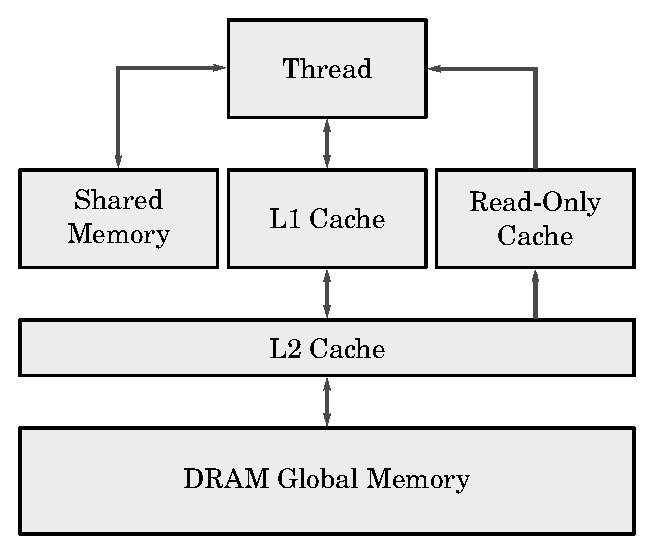
\includegraphics[scale=.62]{./images/GPUthreads.eps}
% \caption{Memory hierarchy of threads in a kernel executed in Kepler architecture}
% \label{fig:GPUthreads}
%\end{figure}

The hierarchical memory of an NVIDIA GPU contains global and shared portions.
Global memory is big, off-chip, has a high latency and can be accessed by all
threads of the kernel.  Shared memory is small, on-chip, has a low-latency and
can be accessed only by threads in a same SM.  Each SM has its own shared L1
cache, and new architectures have coherent global L2 caches.  Optimizing thread
accesses to different memory levels is essential to achieve good performance.
%Figure \ref{fig:GPUthreads} shows the memory access hierarchy in a Kepler
%architecture.

%\begin{table}[htpb]
%\centering
%\small
%\begin{tabular}{| l | c | c | c  |  c | c |}
%\hline \hline%inserts double horizontal lines
% \textbf{Type} & \textit{\textbf{On Chip}}&\textbf{
%Cacheable}&\textbf{Instructions}&\textbf{Visibility}\\ \hline
%Registers&Yes&No&Load/Store&\textit{Thread}\\ \hline
%Shared&Yes&No&Load/Store&Block\\ \hline
%Cache L1&Yes&No&Load/Store&Block\\ \hline
%Constant&No&Yes&Load&\textit{Kernels}\\ \hline
%Texture&No&Yes&Load/Store&\textit{Kernel}\\ \hline
%Local&No&Yes&Load/Store&\textit{Thread}\\ \hline
%Cache L2&No&Yes&Load/Store&\textit{Kernel}\\ \hline
%Global&No&Yes&Load/Store&\textit{Kernel}\\ \hline
%\hline
%\end{tabular}
%\caption{Memory types in GPUs supported by CUDA}
%\label{tab:memories} % is used to refer this table in the text
%\end{table}


\subsubsection{Compute Unified Device Architecture (CUDA)}

The CUDA programming model and platform enables the use of NVIDIA GPUs for
scientific and general purpose computation.  A single \textit{master} thread
runs in the CPU, launching and managing computations on the GPU.  Data for the
computations has to be transferred from the main memory to the GPU's memory.
Multiple computations launched by the master thread, or \textit{kernels}, can
run asynchronously and concurrently. If the threads from a same warp must
execute different instructions the CUDA compiler must generate code to branch
the execution correctly, making the program lose performance due to this
\textit{warp divergence}.

The CUDA language extends C and provides a multi-step compiler, called
\textit{NVCC}, that translates CUDA code to Parallel Thread Execution code, or
\textit{PTX}.  \textit{NVCC} uses the host's C++ compiler in several
compilation steps, and also to generate code to be executed in the host. The
final binary generated by \textit{NVCC} contains code for the GPU and the host.
When \textit{PTX} code is loaded by an application at run-time, it is compiled
to binary code by the host's device driver.  This binary code can be executed
in the device's processing cores, and is architecture-specific.  The targeted
architecture can be specified using \textit{NVCC} parameters.

\subsubsection{GPU Performance Models and Autotuning}

The accuracy of a GPU performance model is subject to low level elements such
as instruction pipeline usage and small cache hierarchies. A GPU's performance
approaches its peak when the instruction pipeline is saturated, but becomes
unpredictable when the pipeline is
under-utilized~\cite{zhang2011quantitative,amaris2015simple}.  Considering the
effects of small cache hierarchies~\cite{dao2015performance,picchi2015impact}
and memory-access
divergence~\cite{sampaio2013divergence,baghsorkhi2010adaptive} is also critical
to a GPU performance model.

Guo and Wang~\cite{guo2010auto} introduce a framework for autotuning
the number of threads and the sizes of blocks and warps used by the CUDA
compiler for sparse matrix and vector multiplication GPU applications.  Li
\emph{et al.}~\cite{li2009note} discuss the performance of autotuning
techniques in highly-tuned GPU General Matrix to Matrix Multiplication (GEMMs)
routines, highlighting the difficulty in developing optimized code for new GPU
architectures.  Grauer-Gray \emph{et al.}~\cite{grauer2012auto}
autotune an optimization space of GPU kernels focusing on tiling, loop
permutation, unrolling, and parallelization.  Chaparala \emph{et
al.}~\cite{chaparala2015autotuning} autotune GPU-accelerated Quadratic
Assignment Problem solvers.  Sedaghati \emph{et
al.}~\cite{sedaghati2015automatic} build a decision model for the selection of
sparse matrix representations in GPUs.

\subsection{Experiments}

This section presents the GPU testbed, the algorithm benchmark, the
autotuner implementation and its search space.

\subsubsection{GPU Testbed}

To be able to show that different GPUs require different options to improve
performance, and that it is possible to achieve speedups in different hardware,
we wanted to tune our benchmark for different NVIDIA microarchitectures.  We
selected the Tesla K40, the GTX 750 and the GTX 980.  Using the GK110B chip,
the Tesla K40 is a Kepler microarchitecture GPU, the oldest GPU of the testbed.
The GTX 750 is the first Maxwell microarchitecture GPU and uses the GM107 chip.
The GTX 980 is the latest Maxwell GPU and uses the GM204 chip.
Table~\ref{tab:GPUs} summarizes the hardware characteristics of the three GPUs.

\begin{table}[thpb]
    \centering
    \footnotesize
    \begin{tabular}{cccccccc}
        \toprule
        \textbf{Model}&\textbf{C.C.}&\textbf{Global Memory}&\textbf{Bus}&\textbf{Bandwidth}&\textbf{L2}&\textbf{Cores/SM}&\textbf{Clock} \\ \midrule
        Tesla-K40&3.5&12 GB&384-bit&276.5 GB/s&1.5 MB&2880/15&745 Mhz \\ \midrule
        GTX-750&5.0&1 GB&128-bit&86.4 GB/s&2 MB&512/4&1110 Mhz \\ \midrule
        GTX-980&5.2&4 GB&256-bit&224.3 GB/s&2 MB&2048/16&1216 Mhz \\ \bottomrule
    \end{tabular}
    \caption{Hardware specifications of the GPUs in the testbed}
    \label{tab:GPUs}
\end{table}

\subsubsection{Algorithm Benchmark}

We composed a benchmark with 17 heterogeneous GPU applications.  The benchmark
contains 4 optimization strategies for \emph{matrix multiplication} (counted as
a single application), 1 vector addition problem, 1 solution for the
\emph{maximum sub-array problem}~\cite{ferreira2014parallel}, 2 \emph{sorting}
algorithms and 12 applications from the Rodinia Benchmark
Suite~\cite{che2009rodinia}.  The remainder of this section discusses some
details of these algorithms, and introduces a three-letter code for each
application, used in section ~\ref{sec:GPUresults}.

\paragraph{Matrix Multiplication} We used four different memory access
optimizations: global memory with non-coalesced accesses (MMU); global memory
with coalesced accesses (MMG); shared memory with non-coalesced accesses to
global memory (MSU); and shared memory with coalesced accesses to global memory
(MMS).  All performance measurements for these optimizations used square
matrices, with $N = 8192$.  The run-time complexity for a sequential matrix
multiplication algorithm using two matrices of size $N\times{}N$ is $O(N^3)$.
In a CUDA application with $N^2$ threads, the run-time complexity is $O(N)$

\paragraph{Vector Addition Algorithm} For two vectors $A$ and $B$, the Vector
Addition (VAD) $C = A + B$ is obtained by adding the corresponding components.
In a GPU algorithm each thread performs an addition of a position of the
vectors $A$ and $B$ and stores the result in the vector $C$.  The number of GPU
threads used in this problem is equal to the size of the vectors.  All
performance measurements for this problem used arrays of size $N = 4194304$.

\paragraph{Maximum Sub-Array Problem} Let $X$ be a sequence of $N$ integer
numbers $(x_1, ... , x_N)$.  The Maximum Sub-Array Problem (MSA) consists of
finding the contiguous sub-array within $X$ which has the largest sum of
elements. The solution for this problem is frequently used in computational
biology for gene identification, analysis of sequences of protein and DNA, and
identification of hydrophobic regions.  The maximum sub-array problem can be
solved sequentially in $O(N)$ comparisons, and in $O(N/t)$
with a parallel solution~\cite{alves2004bsp}, where $t$ is the number of
threads.

The implementation~\cite{ferreira2014parallel} used in this study creates a
kernel with 4096 threads, divided in 32 blocks with 128 threads.  The $N$
elements are divided in intervals of $N/t$, and each block receives a portion
of the array.  The blocks use the shared memory for storing segments, which are
read from the global memory using coalesced accesses. Each interval is reduced
to a set of 5 integer variables, which are stored in vector of size $5 \times
t$ in global memory. This vector is then transferred to the CPU memory for
later processing.  All performance measurements for the Maximum Sub-array
Problem used arrays with $N = 1073741824$.

\paragraph{Sorting Algorithms} The benchmark contains two sorting algorithms,
quicksort (QKS, with $N = 65536$) and bitonicsort (BTN, with $N =
4194304$)~\footnote{Obtained from: \texttt{\scriptsize
http://digitalcommons.providence.edu/student\_scholarship/7/} [Accessed on 10
February 2015]}.  Both algorithms sort random numbers sampled from a uniform
distribution.

\paragraph{Rodinia Benchmark Suite} Rodinia's~\cite{che2009rodinia}
applications have implementations for multi-core CPUs and GPUs using three
parallel programming models (OpenMP, CUDA and OpenCL). The benchmark was
devised for heterogenous parallel computing research and its applications
represent different high-level domains or behaviours, called the Berkeley
dwarfs~\cite{asanovic2006landscape, asanovic2009view}.
Table~\ref{tab:Rodinia} shows the Rodinia applications contained in our
benchmark.

\begin{table}[htpb]
    \centering
    \footnotesize
        \begin{tabular}{ccc}
            \toprule
            \textbf{Application} & \textbf{Berkeley Dwarf\cite{asanovic2009view}} & \textbf{Domain} \\\midrule
            B+Tree (BPT) & Graph Traversal& Search \\\midrule
            Back Propagation (BCK) & Unstructured Grid & Pattern Recognition \\\midrule
            Breadth-First Search (BFS) & Graph Traversal & Graph Algorithms \\\midrule
            Gaussian Elimination (GAU) & Dense Linear Algebra & Linear Algebra \\\midrule
            Heart Wall (HWL) & Structured Grid & Medical Imaging \\\midrule
            Hot Spot (HOT) & Structured Grid & Physics Simulation \\\midrule
            K-Means (KMN) & Dense Linear Algebra & Data Mining \\\midrule
            LavaMD (LMD) & N-Body & Molecular Dynamics \\\midrule
            LU Decomposition (LUD) & Dense Linear Algebra & Linear Algebra \\\midrule
            Myocyte (MYO) & Structured Grid & Biological Simulation \\\midrule
            Needleman-Wunsch (NDL) & Dynamic Programming & Bioinformatics \\\midrule
            Path Finder (PTF) & Dynamic Programming & Grid Traversal \\\bottomrule
        \end{tabular}
    \caption{Rodinia applications used in the experiments}
    \label{tab:Rodinia}
\end{table}

\subsection{The Autotuner}
\label{sec:tuner}

Our implementation uses the OpenTuner framework's native parameter types to
represent CUDA compilation options. Flags and multi-valued parameters are
represented as single \emph{EnumParameter}s, and parameters that accept
numerical values are represented as \emph{IntegerParameter}s.  The same
encoding was used in Jansel \emph{et al.}~\cite{ansel2014opentuner} in the
implementation of an autotuner for GCC compilation parameters.

The autotuner we implemented used the \textit{multi-armed bandit with sliding
window, area under the curve credit assignment} meta-technique, simply named
\textit{AUC Bandit}.  AUC Bandit is OpenTuner's core
meta-technique~\cite{ansel2014opentuner}, and its ensemble of search techniques
is composed by implementations of the Nelder-Mead algorithm and three
variations of genetic algorithms.  There is no guarantee that any tuning run
will find the optimal solution, but the variance of the results found by
different tuning runs decreases as tuning time progresses, as is shown in the
results from the original OpenTuner paper~\cite{ansel2014opentuner}.

The search in the space of CUDA options potentially generates invalid parameter
combinations due to incompatible flags or architecture restrictions.  To
prevent these invalid configurations from misguiding the search techniques we
first modified all programs in the benchmark so that they verify the
correctness of their output using previously computed correct outputs. Then we
made the autotuner check for errors during compilation and execution whenever
testing a new configuration and assign a penalty value when finding errors.
Errors could be used to acquire knowledge about the interactions and
incompatibilities between parameters, which would enable the autotuner to prune
the search space and find better solutions faster.  The final verification step
used to validate an autotuned result was to manually check the output of the
CUDA toolkit's \texttt{nvprof} profiler, certifying that the CUDA kernels were
launched and executed properly.

The code for our autotuner and all the experiments and results is
available\footnote{Hosted at GitHub: \texttt{\scriptsize
https://github.com/phrb/gpu-autotuning} [Accessed on 10 February 2015]} under
the GNU General Public License.

\subsection{The Search Space}
\label{sec:parameters}

\newcommand{\specialcell}[1]{\begin{minipage}[m]{0.52\columnwidth}\centering#1\end{minipage}}

\begin{table}[htpb]
    \centering
    \footnotesize
        \begin{tabular}{cc}
        \toprule
        \textbf{Flag}&\textbf{Description} \\\midrule
        \texttt{no-align-double} & \specialcell{Specifies that \texttt{malign-double} should not be passed as a compiler argument on 32-bit platforms. \textbf{Step}: NVCC} \\ \midrule
        \texttt{use\_fast\_math} & \specialcell{Uses the fast math library, implies \texttt{ftz=true}, \texttt{prec-div=false}, \texttt{prec-sqrt=false} and \texttt{fmad=true}. \textbf{Step}: NVCC} \\\midrule
        \texttt{gpu-architecture} & \specialcell{Specifies the NVIDIA virtual GPU architecture for which the CUDA input files must be compiled. \textbf{Step}: NVCC \textbf{Values}: \texttt{sm\_20}, \texttt{sm\_21}, \texttt{sm\_30}, \texttt{sm\_32}, \texttt{sm\_35}, \texttt{sm\_50}, \texttt{sm\_52}} \\\midrule
        \texttt{relocatable-device-code} & \specialcell{Enables the generation of relocatable device code. If disabled, executable device code is generated. Relocatable device code must be linked before it can be executed. \textbf{Step}: NVCC} \\\midrule
        \texttt{ftz} & \specialcell{Controls single-precision denormals support. \texttt{ftz=true} flushes denormal values to zero and \texttt{ftz=false} preserves denormal values. \textbf{Step}: NVCC} \\\midrule
        \texttt{prec-div} & \specialcell{Controls single-precision floating-point division and reciprocals. \texttt{prec-div=true} enables the IEEE round-to-nearest mode and \texttt{prec-div=false} enables the fast approximation mode. \textbf{Step}: NVCC} \\\midrule
        \texttt{prec-sqrt} & \specialcell{Controls single-precision floating-point squre root. \texttt{prec-sqrt=true} enables the IEEE round-to-nearest mode and \texttt{prec-sqrt=false} enables the fast approximation mode. \textbf{Step}: NVCC} \\\midrule
        \texttt{def-load-cache} & \specialcell{Default cache modifier on global/generic load. \textbf{Step}: PTX \textbf{Values}: \texttt{ca}, \texttt{cg}, \texttt{cv}, \texttt{cs}} \\\midrule
        \texttt{opt-level} & \specialcell{Specifies high-level optimizations. \textbf{Step}: PTX \textbf{Values}: \texttt{0 - 3}} \\\midrule
        \texttt{fmad} & \specialcell{Enables the contraction of floating-point multiplies and adds/subtracts into floating-point multiply-add operations (FMAD, FFMA, or DFMA). \textbf{Step}: PTX} \\\midrule
        \texttt{allow-expensive-optimizations} & \specialcell{Enables the compiler to perform expensive optimizations using maximum available resources (memory and compile-time). If unspecified, default behavior is to enable this feature for optimization level $\geqslant$O2. \textbf{Step}: PTX} \\\midrule
        \texttt{maxrregcount} & \specialcell{Specifies the maximum number of registers that GPU functions can use. \textbf{Step}: PTX \textbf{Values}: \texttt{16 - 64}} \\\midrule
        \texttt{preserve-relocs} & \specialcell{Makes the \texttt{PTX} assembler generate relocatable references for variables and preserve relocations generated for them in the linked executable. \textbf{Step}: NVLINK} \\\midrule
        \end{tabular}
    \caption{Description of flags in the search space}
    \label{tab:flags}
\end{table}

Table~\ref{tab:flags} details the subset of the CUDA configuration parameters
used in the experiments~\footnote{Adapted from:
http://docs.nvidia.com/cuda/cuda-compiler-driver-nvcc [Accessed on 10 February
2015]}.  The parameters target different compilation steps: the \emph{PTX}
optimizing assembler; the \emph{NVLINK} linker; and the \emph{NVCC} compiler.
We compared the performance of programs generated by tuned parameters with the
standard compiler optimizations, namely \texttt{--opt-level=0,1,2,3}.
Different \texttt{--opt-level}s could also be selected during tuning.  We did
not use compiler options that target the host linker or the library manager
since they do not affect performance.  The size of the search space defined by
all possible combinations of the flags in Table~\ref{tab:flags} is in the order
of $10^{6}$ making hand-optimization or exhaustive searches very time
consuming.

\subsection{Results}
\label{sec:GPUresults}

This section presents the speedups achieved for all algorithms in the
application benchmark, highlights the most significant speedups, and discusses
the performance and accuracy of the autotuner.

\subsubsection{Performance Improvements}

All boxplots presented in this section were made using the standard
implementations available for the R language.  The black band inside the boxes
represents the median of the measurements. The lower and upper bounds of the
box represent, respectively, the first and third quartiles of the data. The
whiskers represent the third and first quartile plus and minus the \emph{inner
quartile range} times 1.5. Finally, the circles represent the outliers.

Figures~\ref{fig:K40hwl}, \ref{fig:980gau}, \ref{fig:K40ptf} and
\ref{fig:K40myo} compare the distributions of 10 perfomance measurements of
binaries compiled with high-level compiler optimizations and with autotuned
compiler options. The results for the high-level optimizations
\texttt{--opt-level=0,1,2,3} were denoted by \emph{-O0}, \emph{-O1}, \emph{-O2}
and \emph{-O3}.  The results for the autotuned configurations were denoted by
the keyword \emph{Tuned}.

\begin{figure}[htpb]
    \centering
    \begin{minipage}{.48\textwidth}
        \centering
        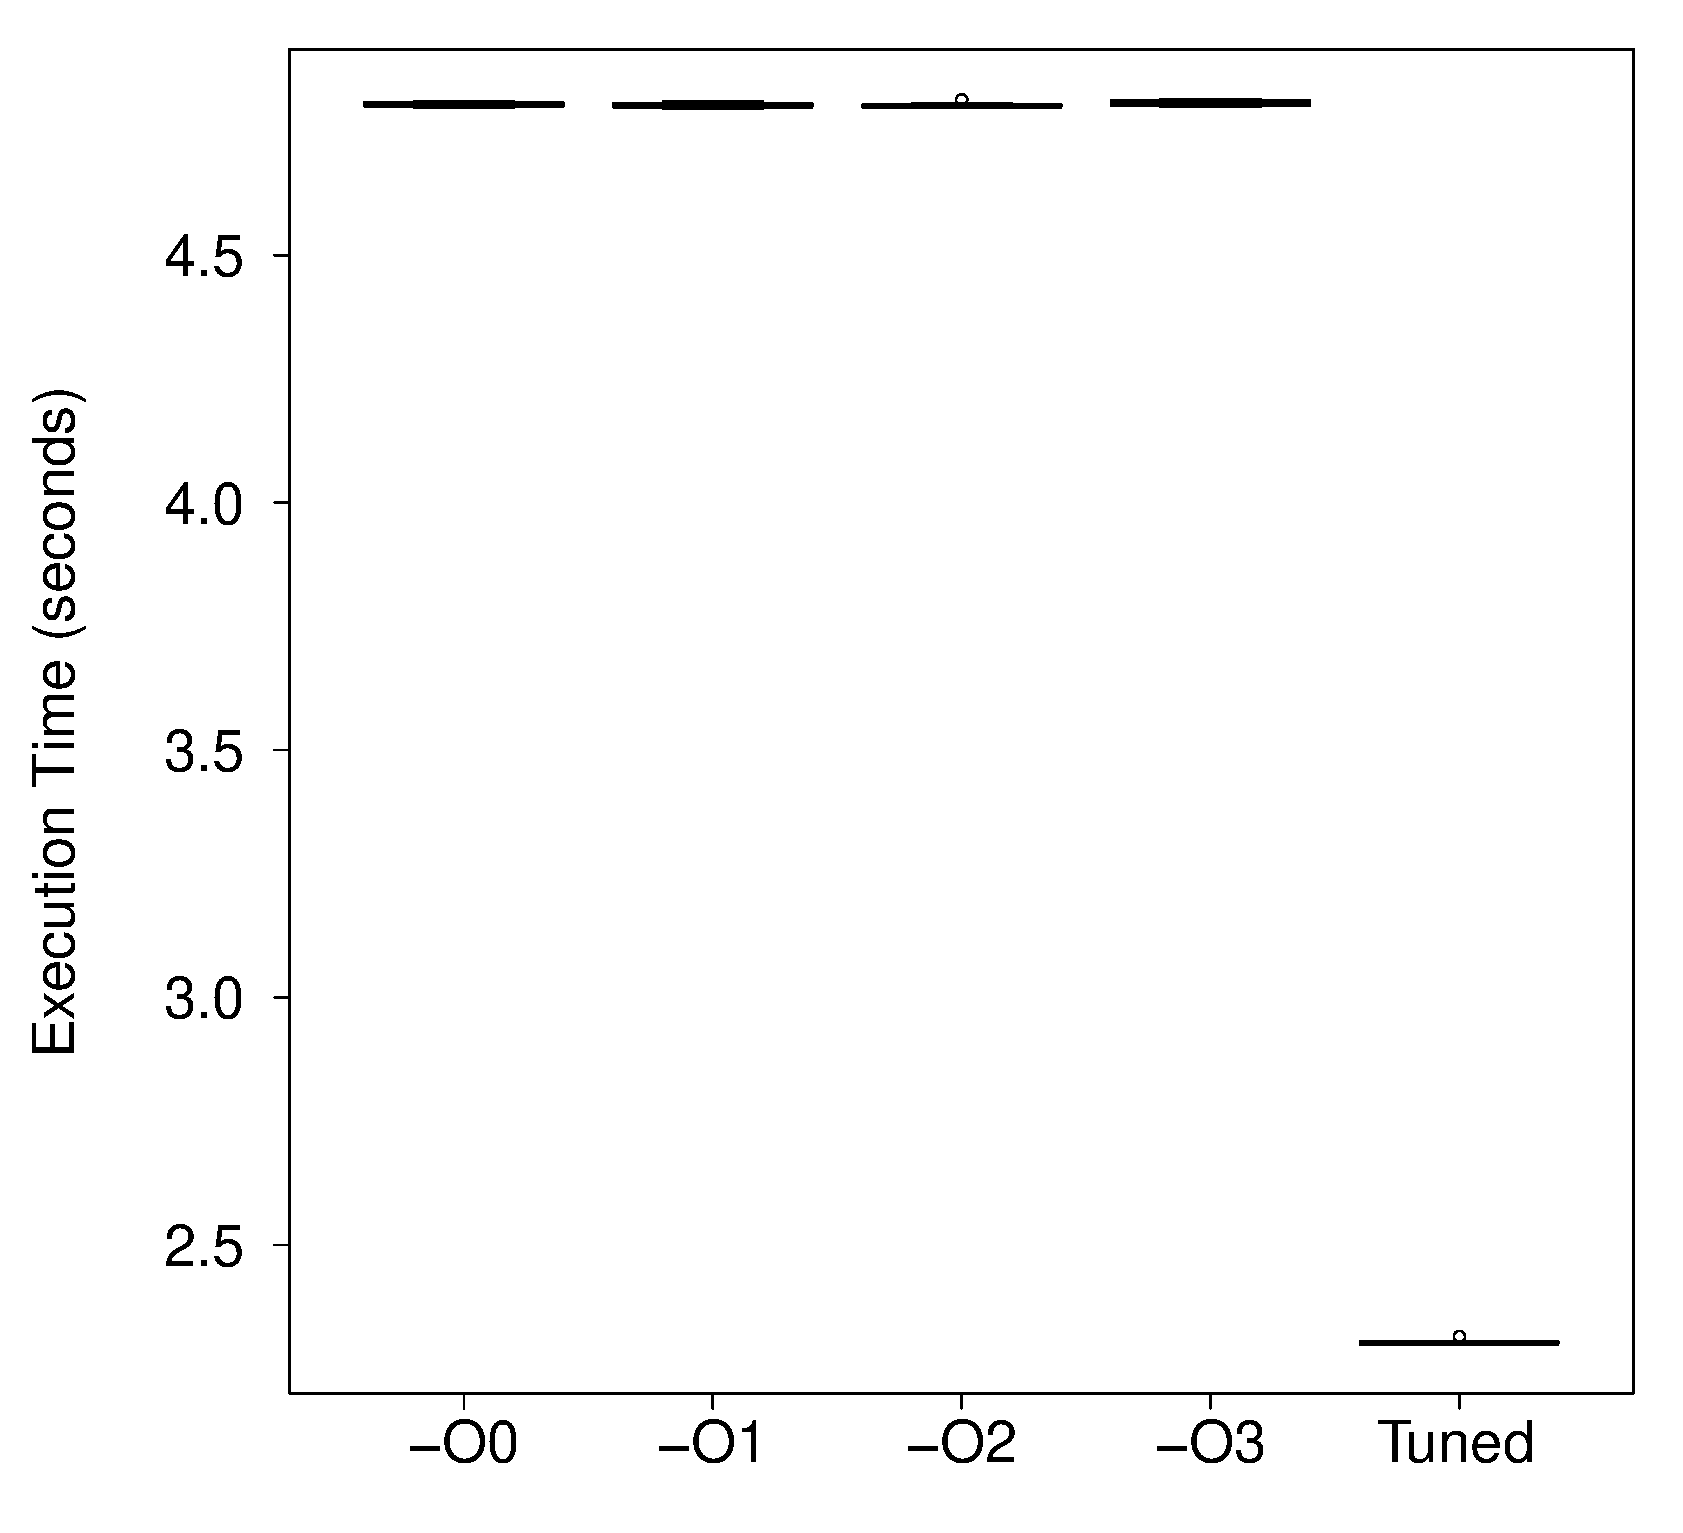
\includegraphics[scale=.22]{./images/heartwall-0-Tesla-K40-Box.eps}
        \caption{Boxplots for the Tesla K40, comparing autotuned results and high-level compiler optimizations for the Heart Wall problem (HWL)}
        \label{fig:K40hwl}
    \end{minipage}%
    \hfill
    \begin{minipage}{.48\textwidth}
        \centering
        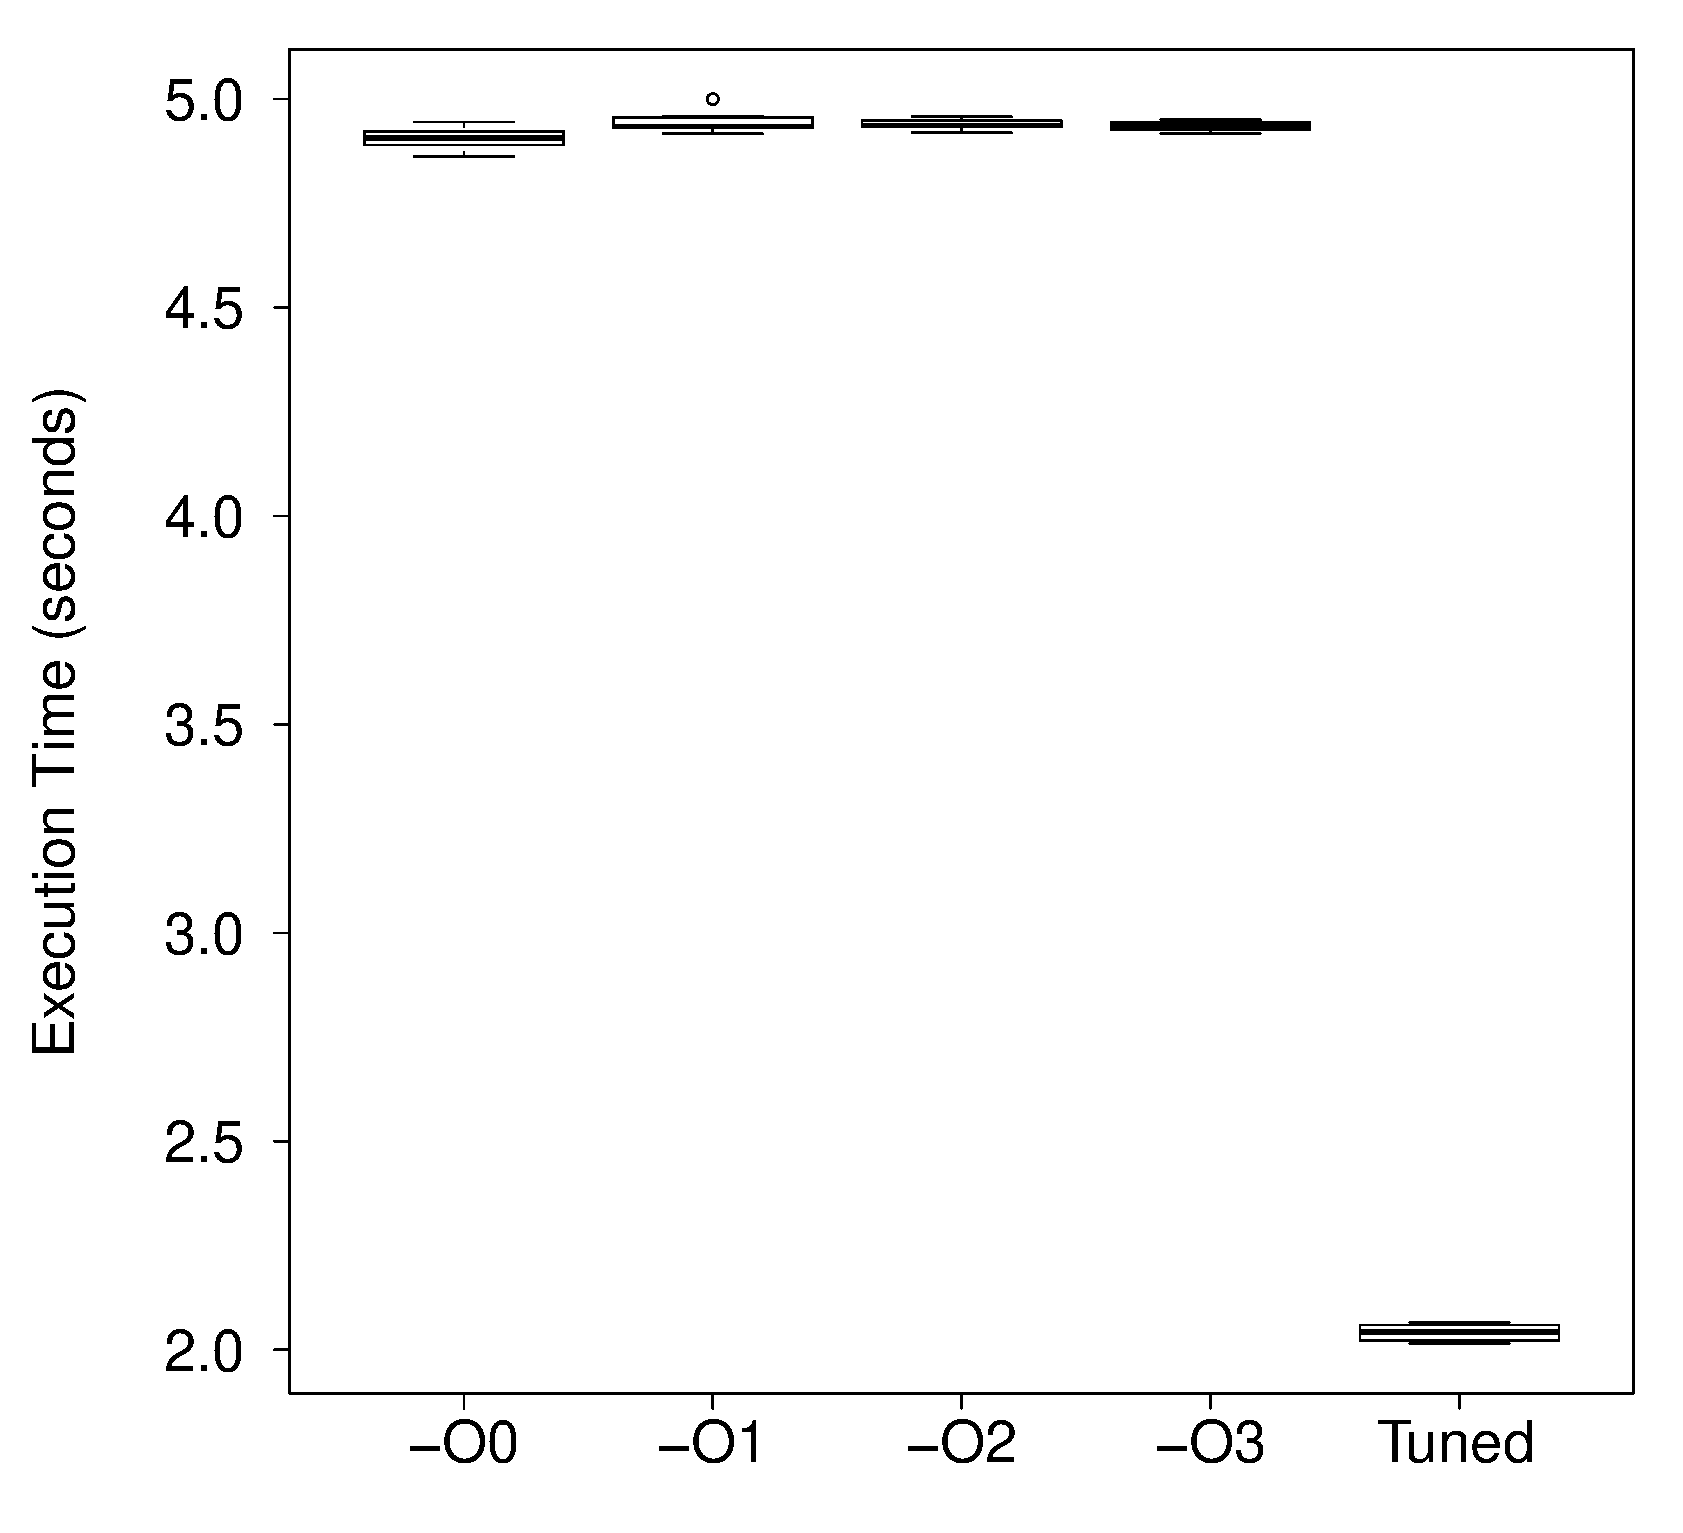
\includegraphics[scale=.22]{./images/gaussian-0-GTX-980-Box.eps}
        \caption{Boxplots for the GTX 980 GPU, comparing autotuned results and high-level compiler optimizations for the Gaussian Elimination problem (GAU)}
        \label{fig:980gau}
    \end{minipage}%

    \begin{minipage}{.48\textwidth}
        \centering
        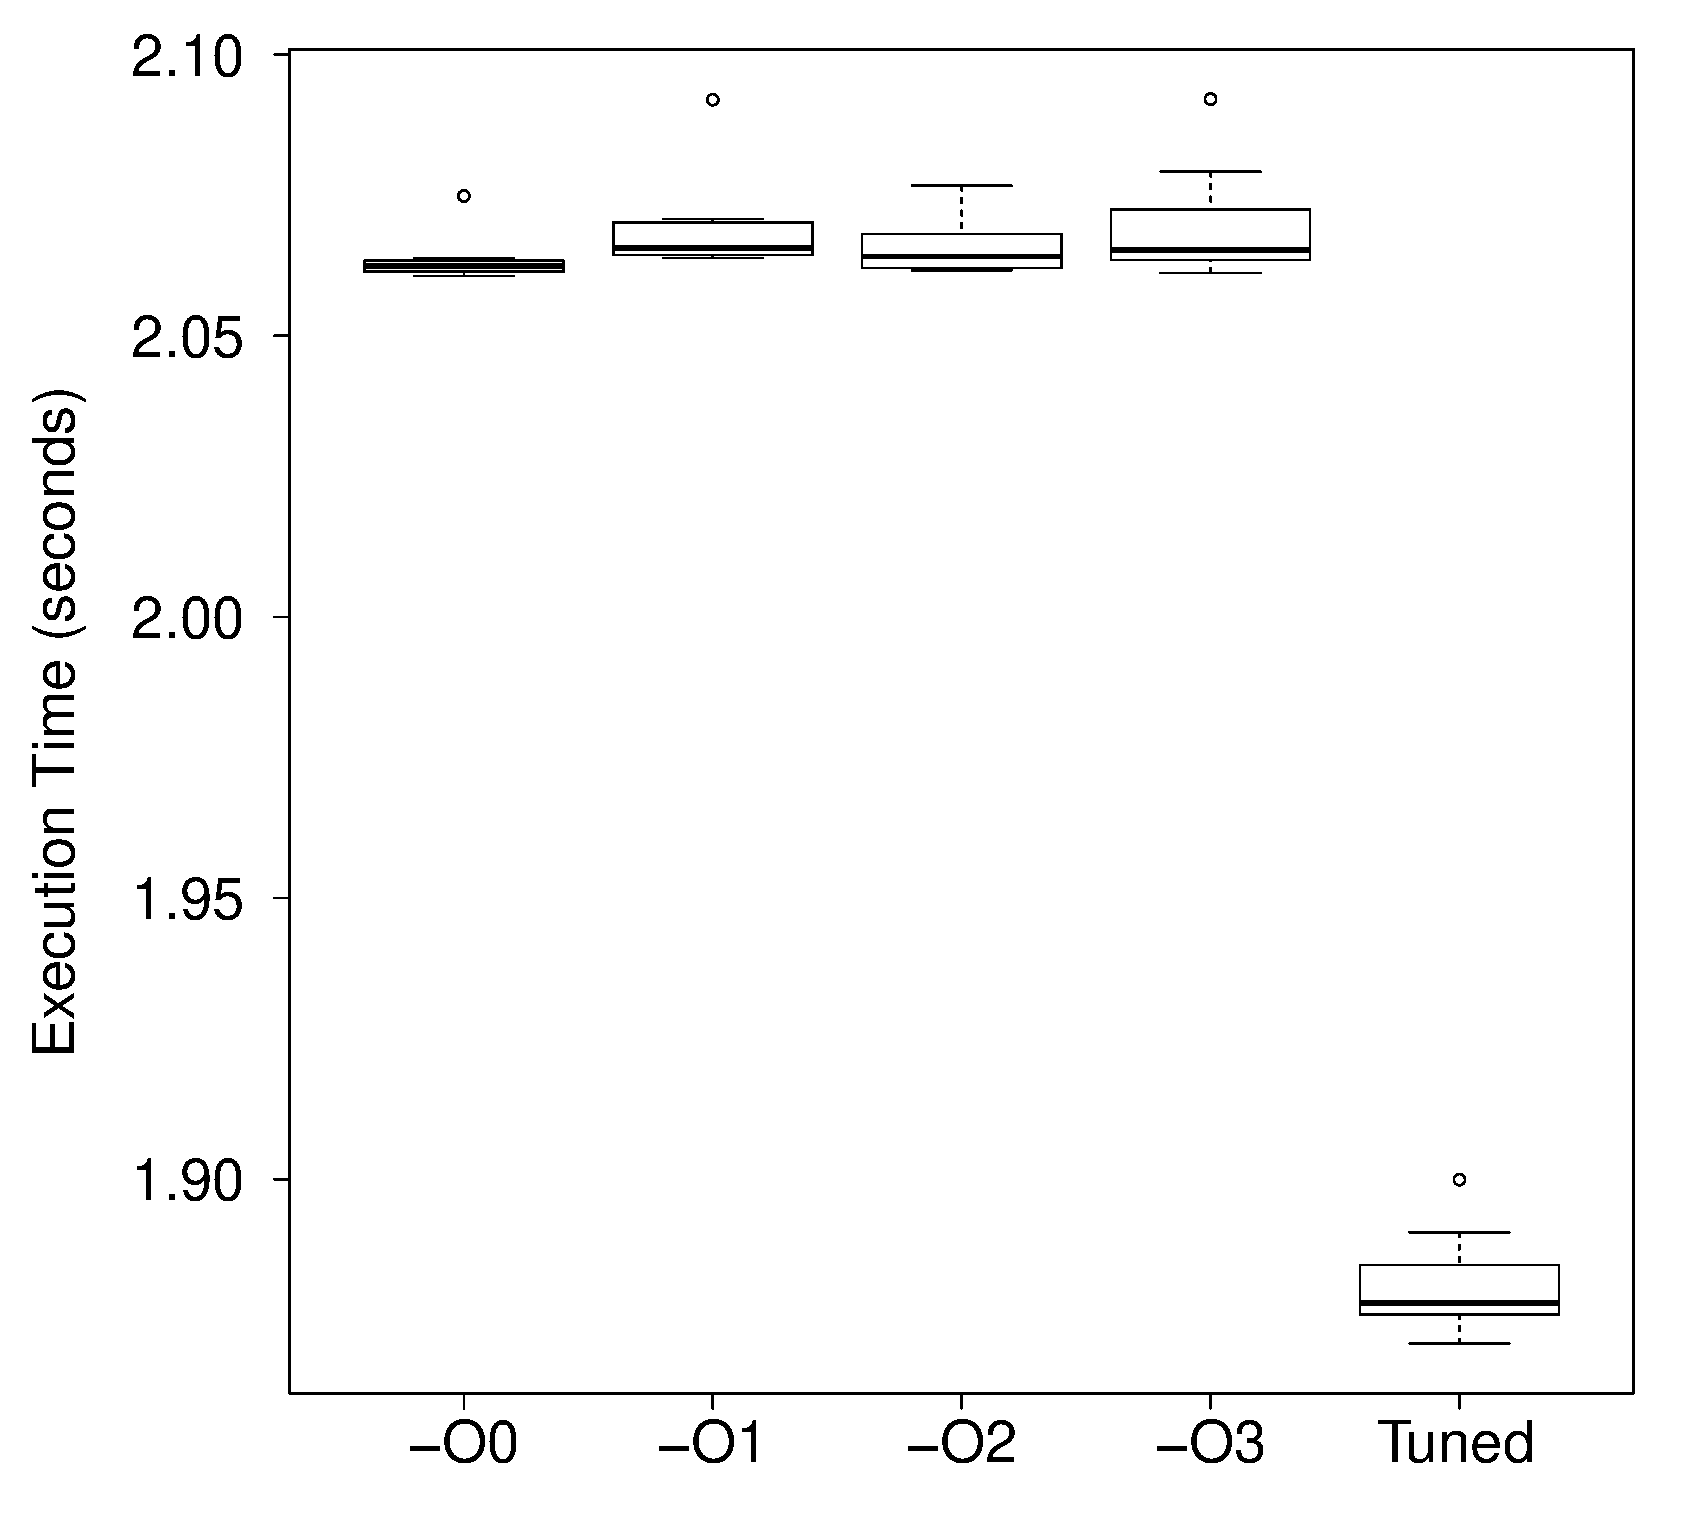
\includegraphics[scale=.22]{./images/Pathfinder-0-Tesla-K40-Box.eps}
        \caption{Boxplots for the Tesla K40, comparing autotuned results and high-level compiler optimizations for the Path Finder problem (PTF)}
        \label{fig:K40ptf}
    \end{minipage}%
    \hfill
    \begin{minipage}{.48\textwidth}
        \centering
        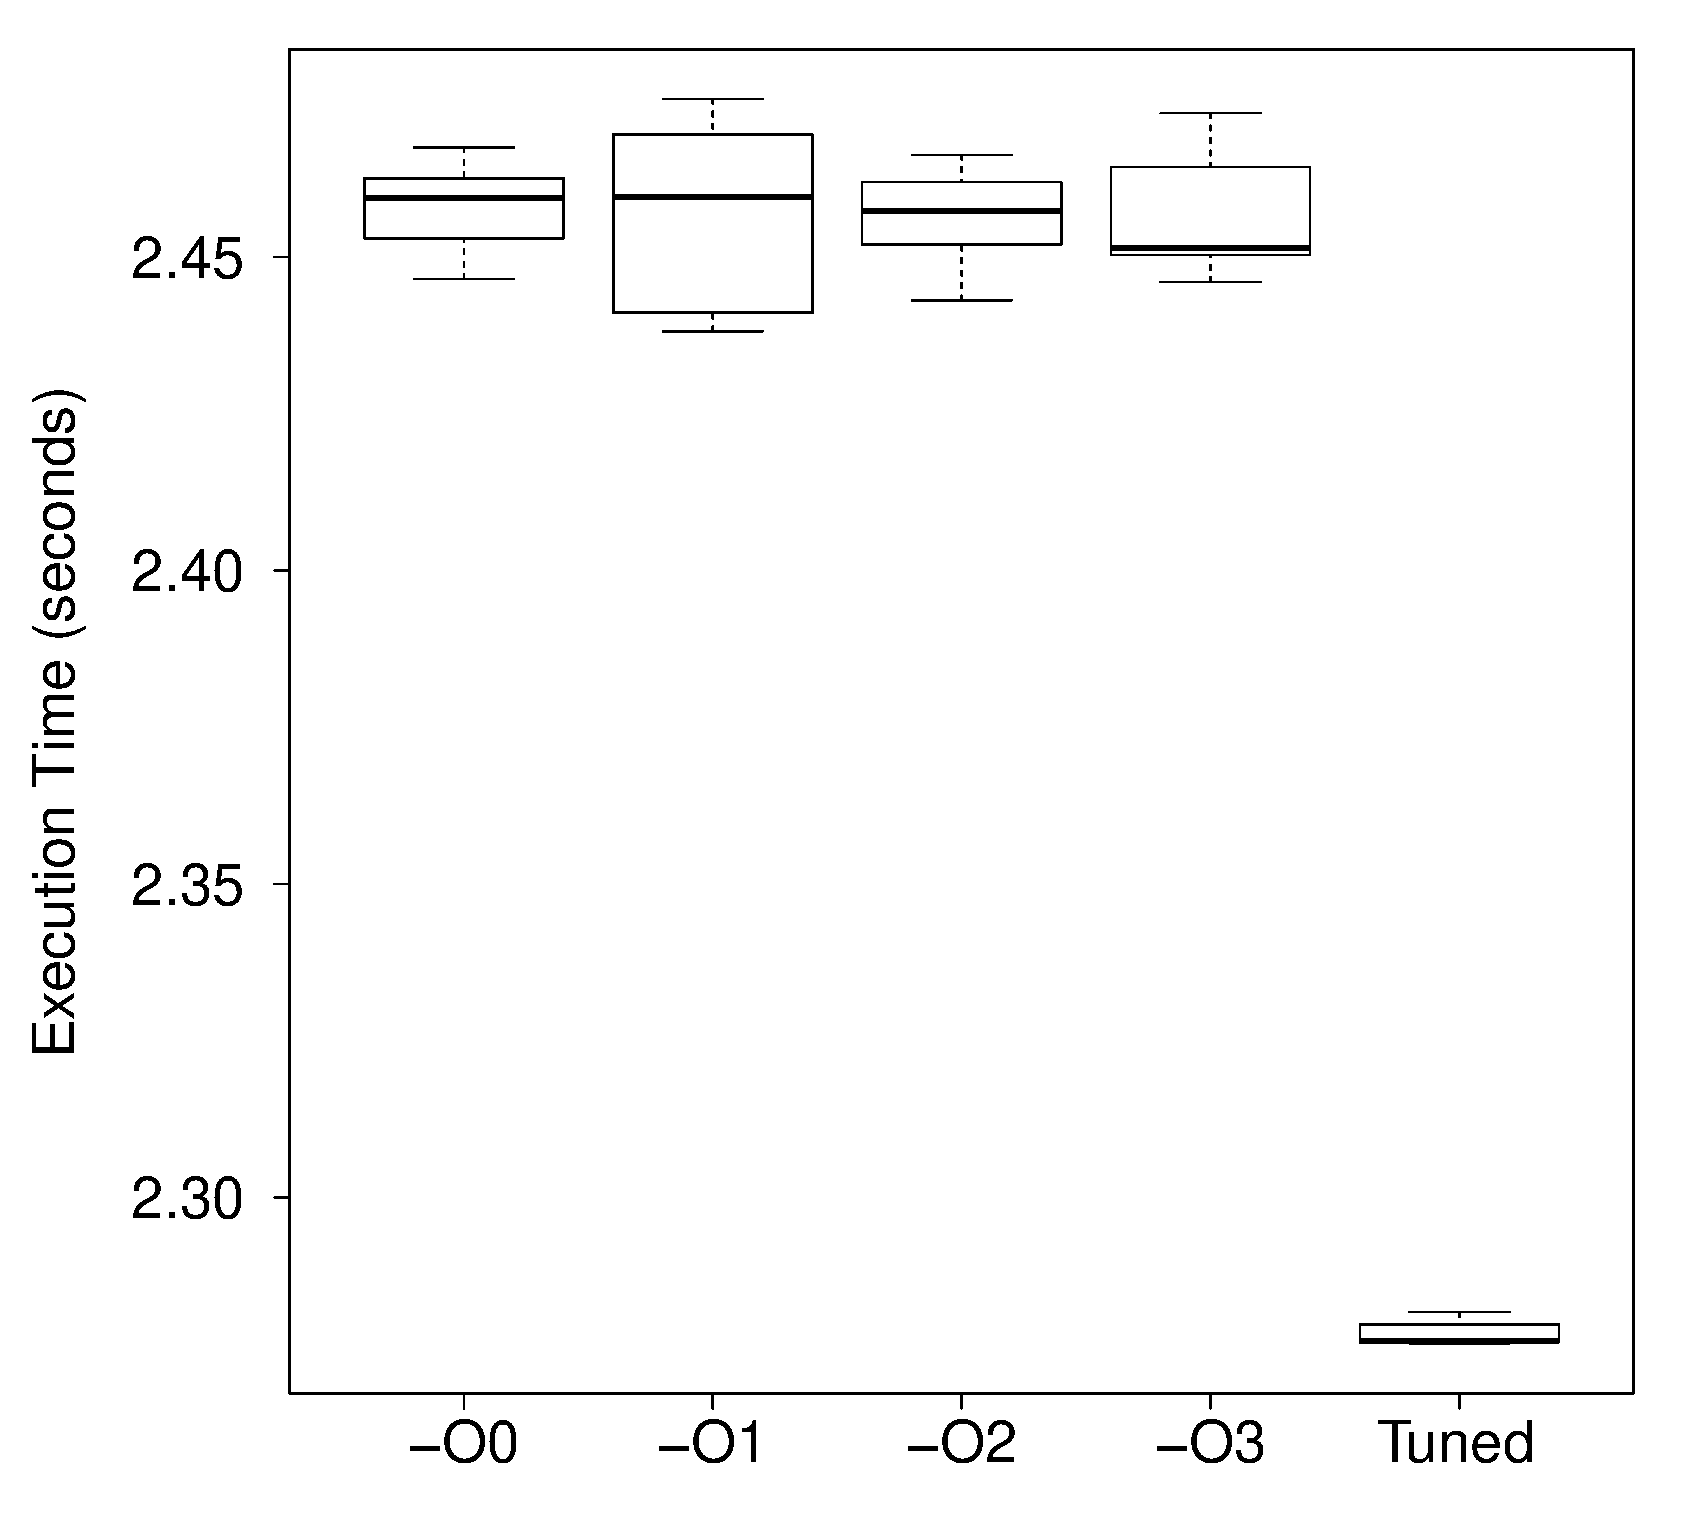
\includegraphics[scale=.22]{./images/myocyte-0-Tesla-K40-Box.eps}
        \caption{Boxplots for the Tesla K40, comparing autotuned results and high-level compiler optimizations for the Myocyte problem (MYO)}
        \label{fig:K40myo}
    \end{minipage}%
\end{figure}

Figure~\ref{fig:K40hwl} shows that the autotuned solution for the Heart Wall
problem (HWL) in the Tesla K40 achieved over 2x speedup in comparison with the
high-level CUDA optimizations.  Figure~\ref{fig:980gau} shows, in the GTX 980,
almost 2.5x speedup for the Gaussian Elimination problem (GAU).
Figure~\ref{fig:K40ptf} show 10\% speedup of the autotuned solution for the
Path Finder problem (PTF) in the Tesla K40.  Figure~\ref{fig:K40myo} shows over
5\% speedup of the autotuned solution, also in the Tesla K40, for the Myocyte
problem (MYO).

Figures~\ref{fig:matrixsummary}, \ref{fig:summary}, \ref{fig:rodiniasummary}
and \ref{fig:rodiniasummarysmall} present summaries of the results. The
autotuner did not find solutions that improved upon the high-level
optimizations for the problems BTN and MSU in any of the GPUs of the testbed,
but it found solutions that achieved speedups for at least one GPU for the
other problems.

\begin{figure}[htpb]
    \centering
    \begin{minipage}{.48\textwidth}
        \centering
        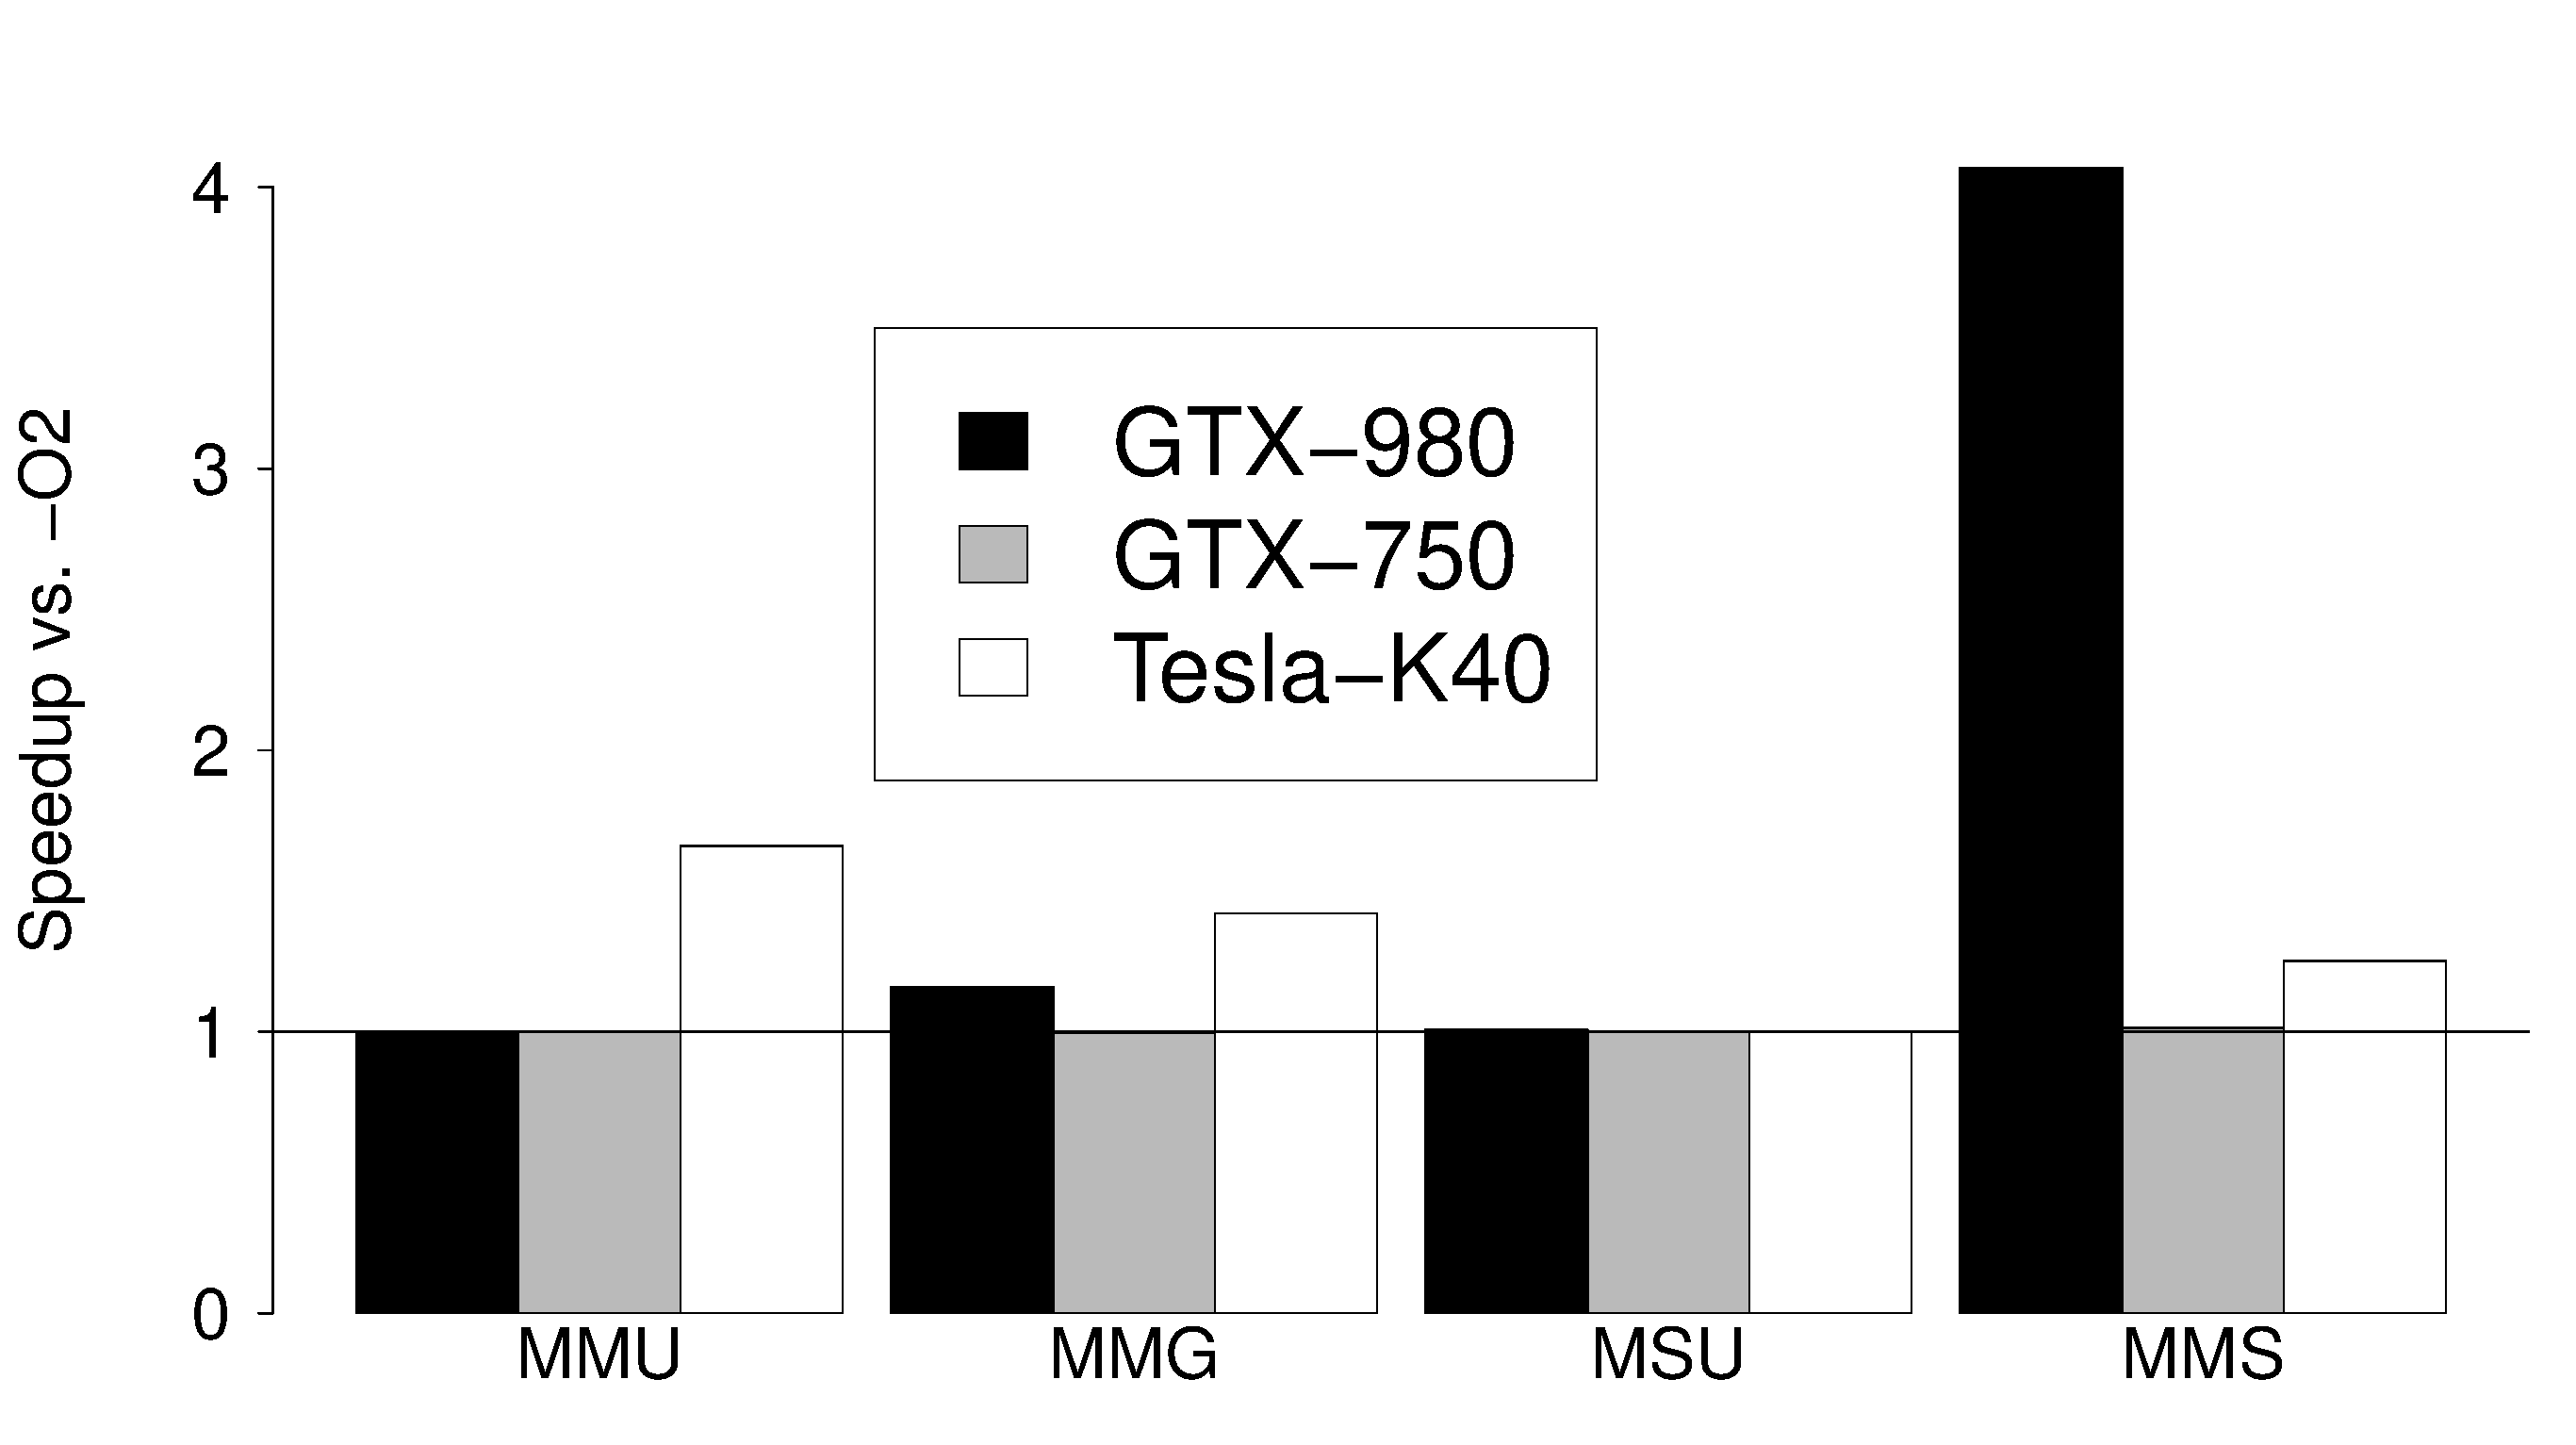
\includegraphics[scale=.15]{./images/MatrixSummary.eps}
        \caption{Summary of the speedups achieved versus \emph{-O2} in the matrix multiplication optimizations}
        \label{fig:matrixsummary}
    \end{minipage}%
    \hfill
    \begin{minipage}{.48\textwidth}
        \centering
        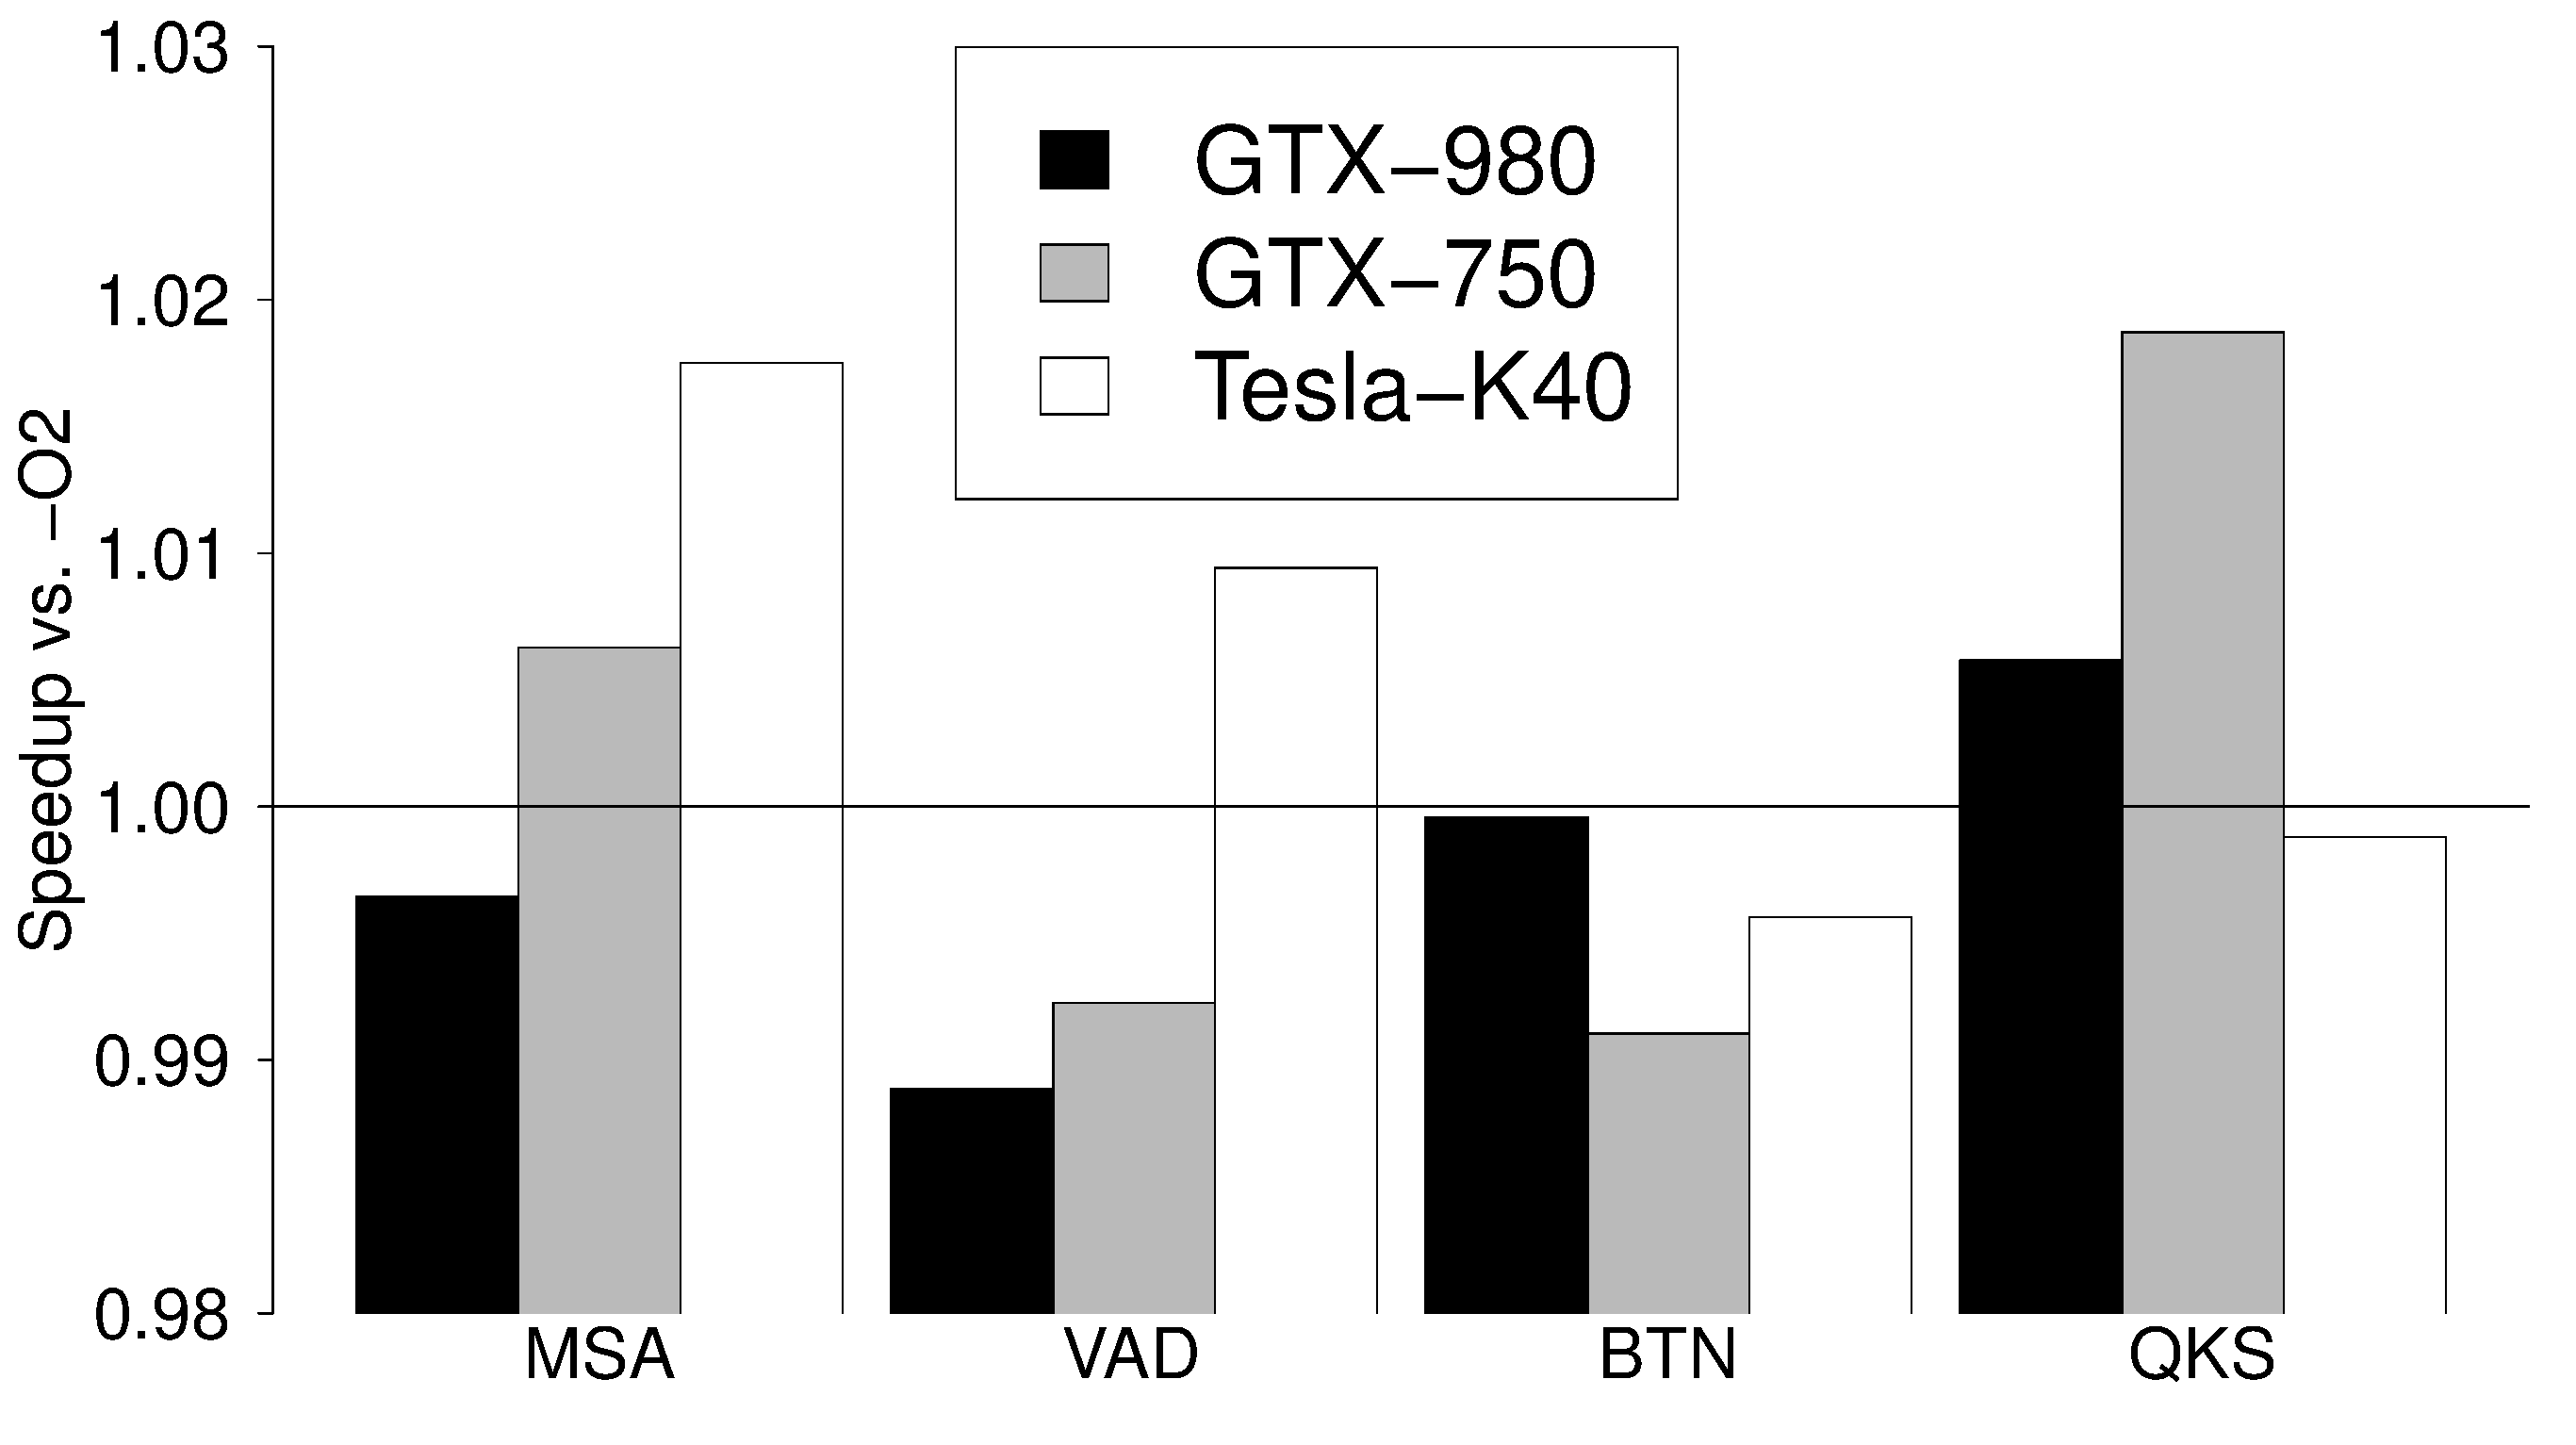
\includegraphics[scale=.15]{./images/Summary.eps}
        \caption{Summary of the speedups achieved versus \emph{-O2} in the other independent applications}
        \label{fig:summary}
    \end{minipage}%
    \hfill
    \begin{minipage}{\textwidth}
        \centering
        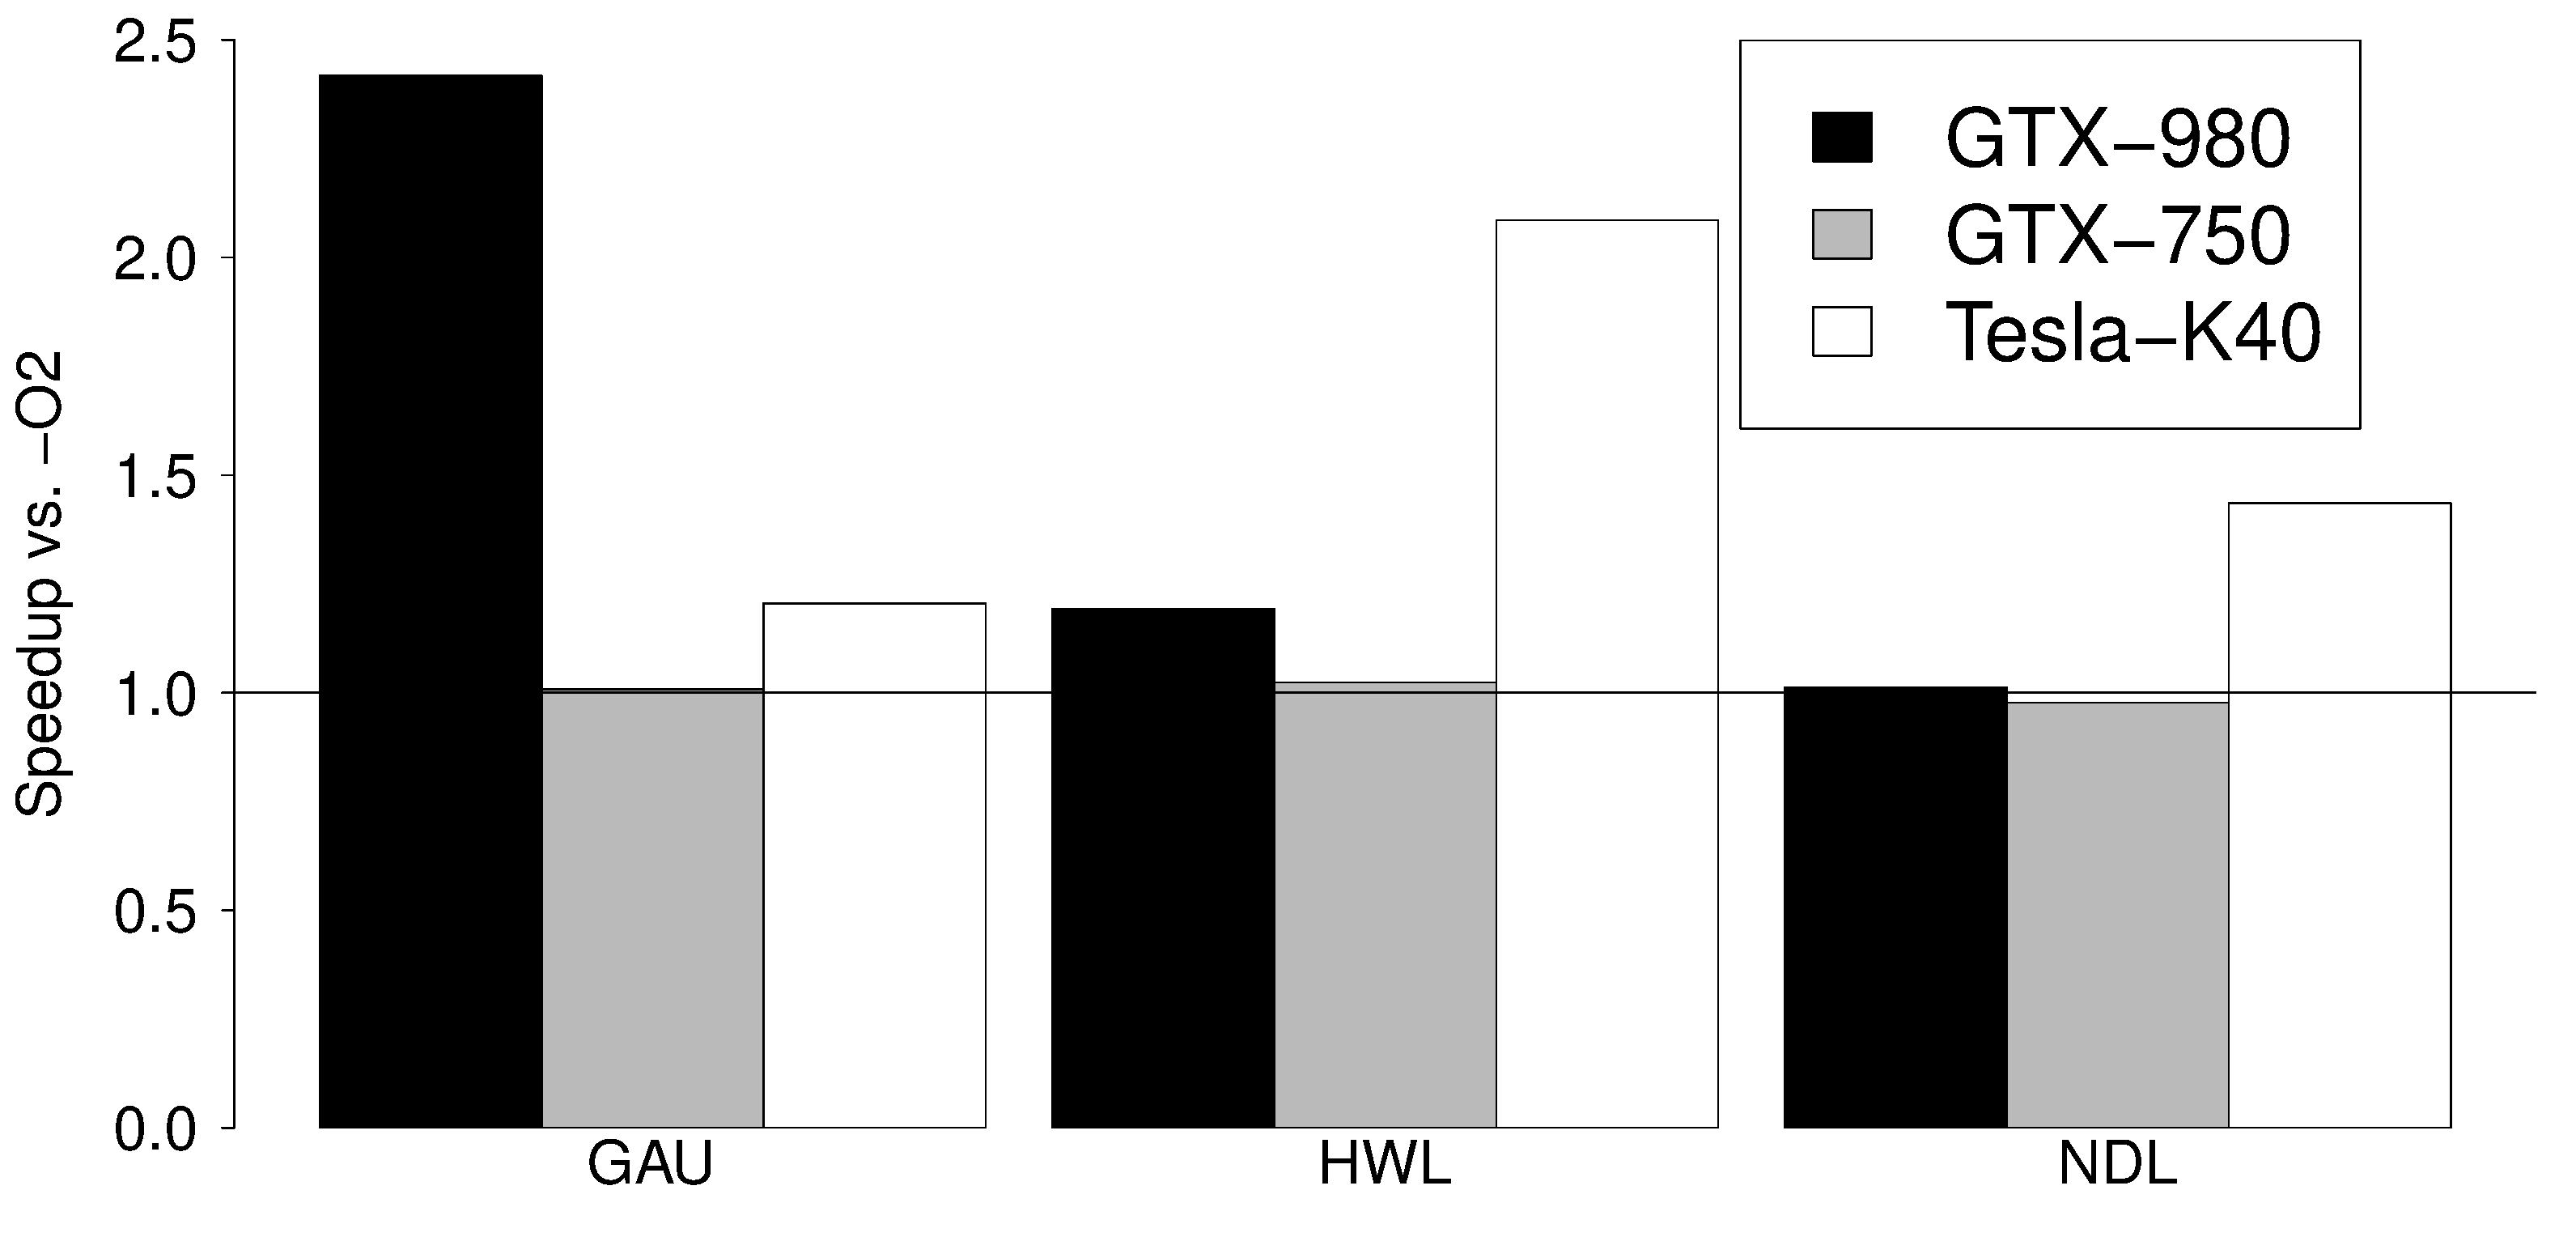
\includegraphics[scale=.15]{./images/RodiniaSummary.eps}
        \caption{Summary of the biggest speedups achieved versus \emph{-O2} in the Rodinia applications}
        \label{fig:rodiniasummary}
    \end{minipage}%

    \begin{minipage}{\textwidth}
        \centering
        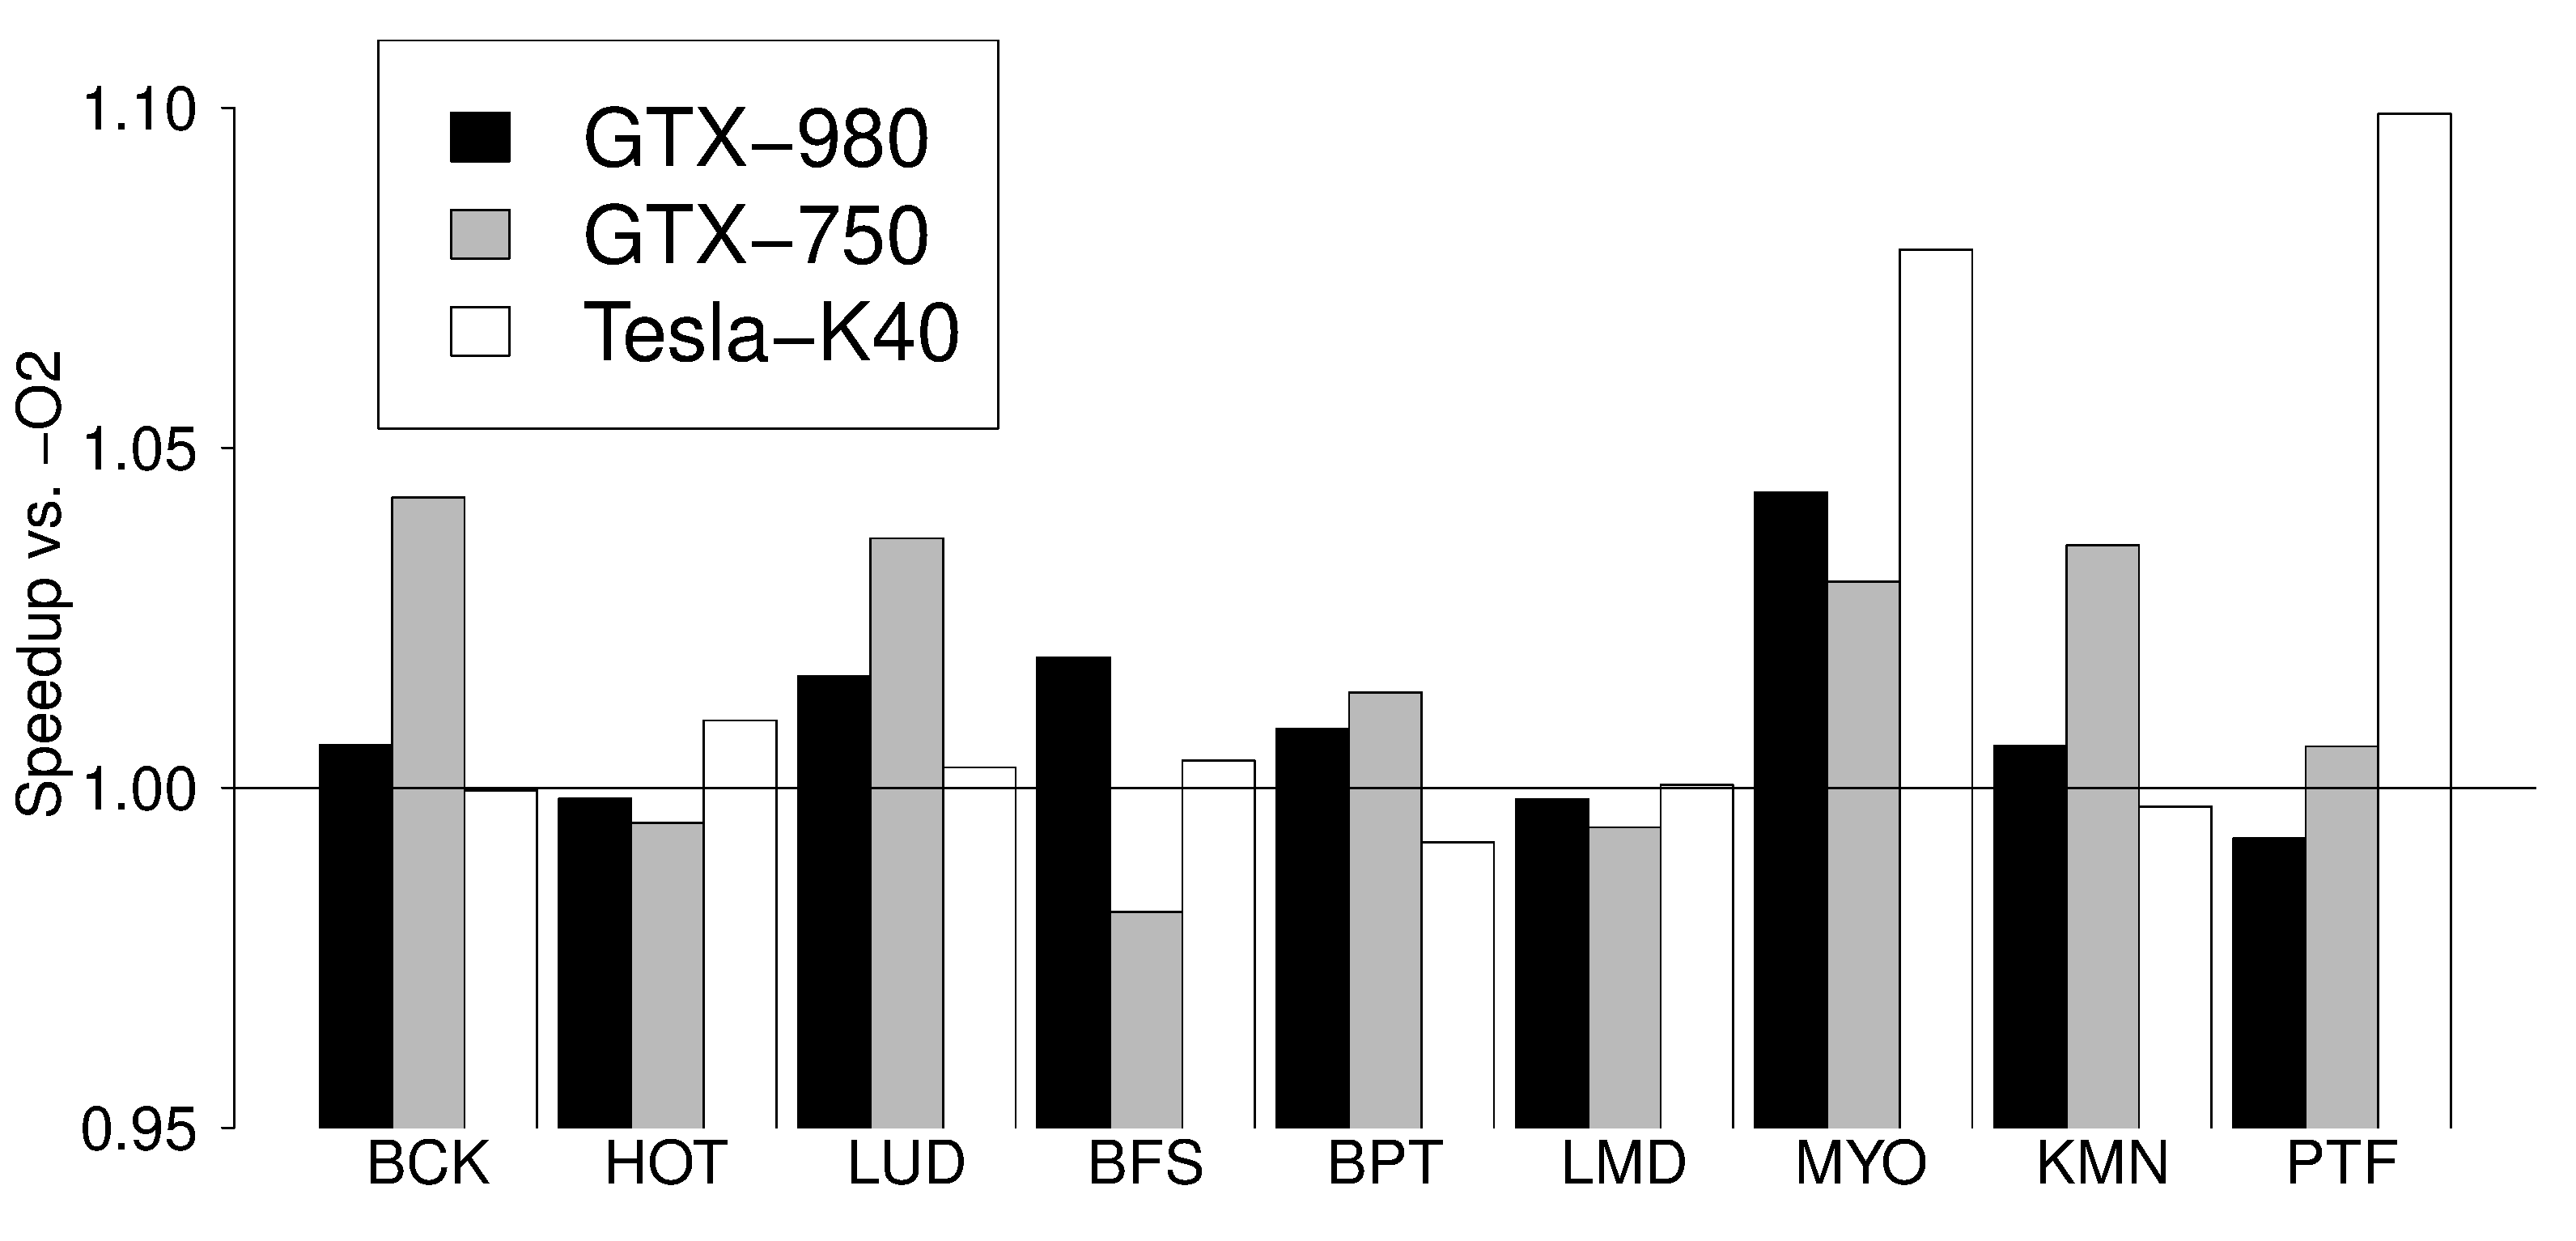
\includegraphics[scale=.15]{./images/RodiniaSummary_small.eps}
        \caption{Summary of the smaller speedups achieved versus \emph{-O2} in the Rodinia applications}
        \label{fig:rodiniasummarysmall}
    \end{minipage}%
\end{figure}

We do not know precisely which hardware characteristics impacted performance
the most.  Although more experiments are needed to confirm the following
hypothesis, we believe that the Maxwell GPUs, the GTX 980 and GTX 750, had
differing results from the Tesla K40 because they are consumer grade GPUs,
producing not so precise results and with different default optimizations. The
similarities between the compute capabilities of the GTX GPUs could also
explain the observed differences from the K40. Finally, the overall greater
computing power of the GTX 980 could explain its differing results from the GTX
750, since the GTX 980 has a greater number of Cores, SMs/Cores, Bandwidth,
Bus, Clock and Global Memory.

\subsubsection{Autotuner Performance}

This section presents an assessment of the autotuner's performance.
Figures~\ref{fig:K40hwBest}, \ref{fig:980gauBest}, \ref{fig:K40ptfBest} and
\ref{fig:K40myoBest} present the performance of the best solution found by the
autotuner versus the time these solutions were found, in seconds since the
beginning of the tuning process. The Figures show the evolution of the
autotuned solution for the best results in our experiments, the Heart Wall
problem (HWL) and the Gaussian Elimination problem (GAU) in the GTX 980, and
the Path Finder problem (PTF) and the Myocyte problem (MYO) in the Tesla K40.

The points in each graph represent the performance, in the y-axis, of the best
configuration found at the corresponding tuning time, shown in the x-axis. The
leftmost point in each graph represents the performance of a configuration
chosen at random by the autotuner. Each subsequent point represents the
performance of the best configuration found so far.

\begin{figure}[htpb]
    \centering
    \begin{minipage}{.48\textwidth}
        \centering
        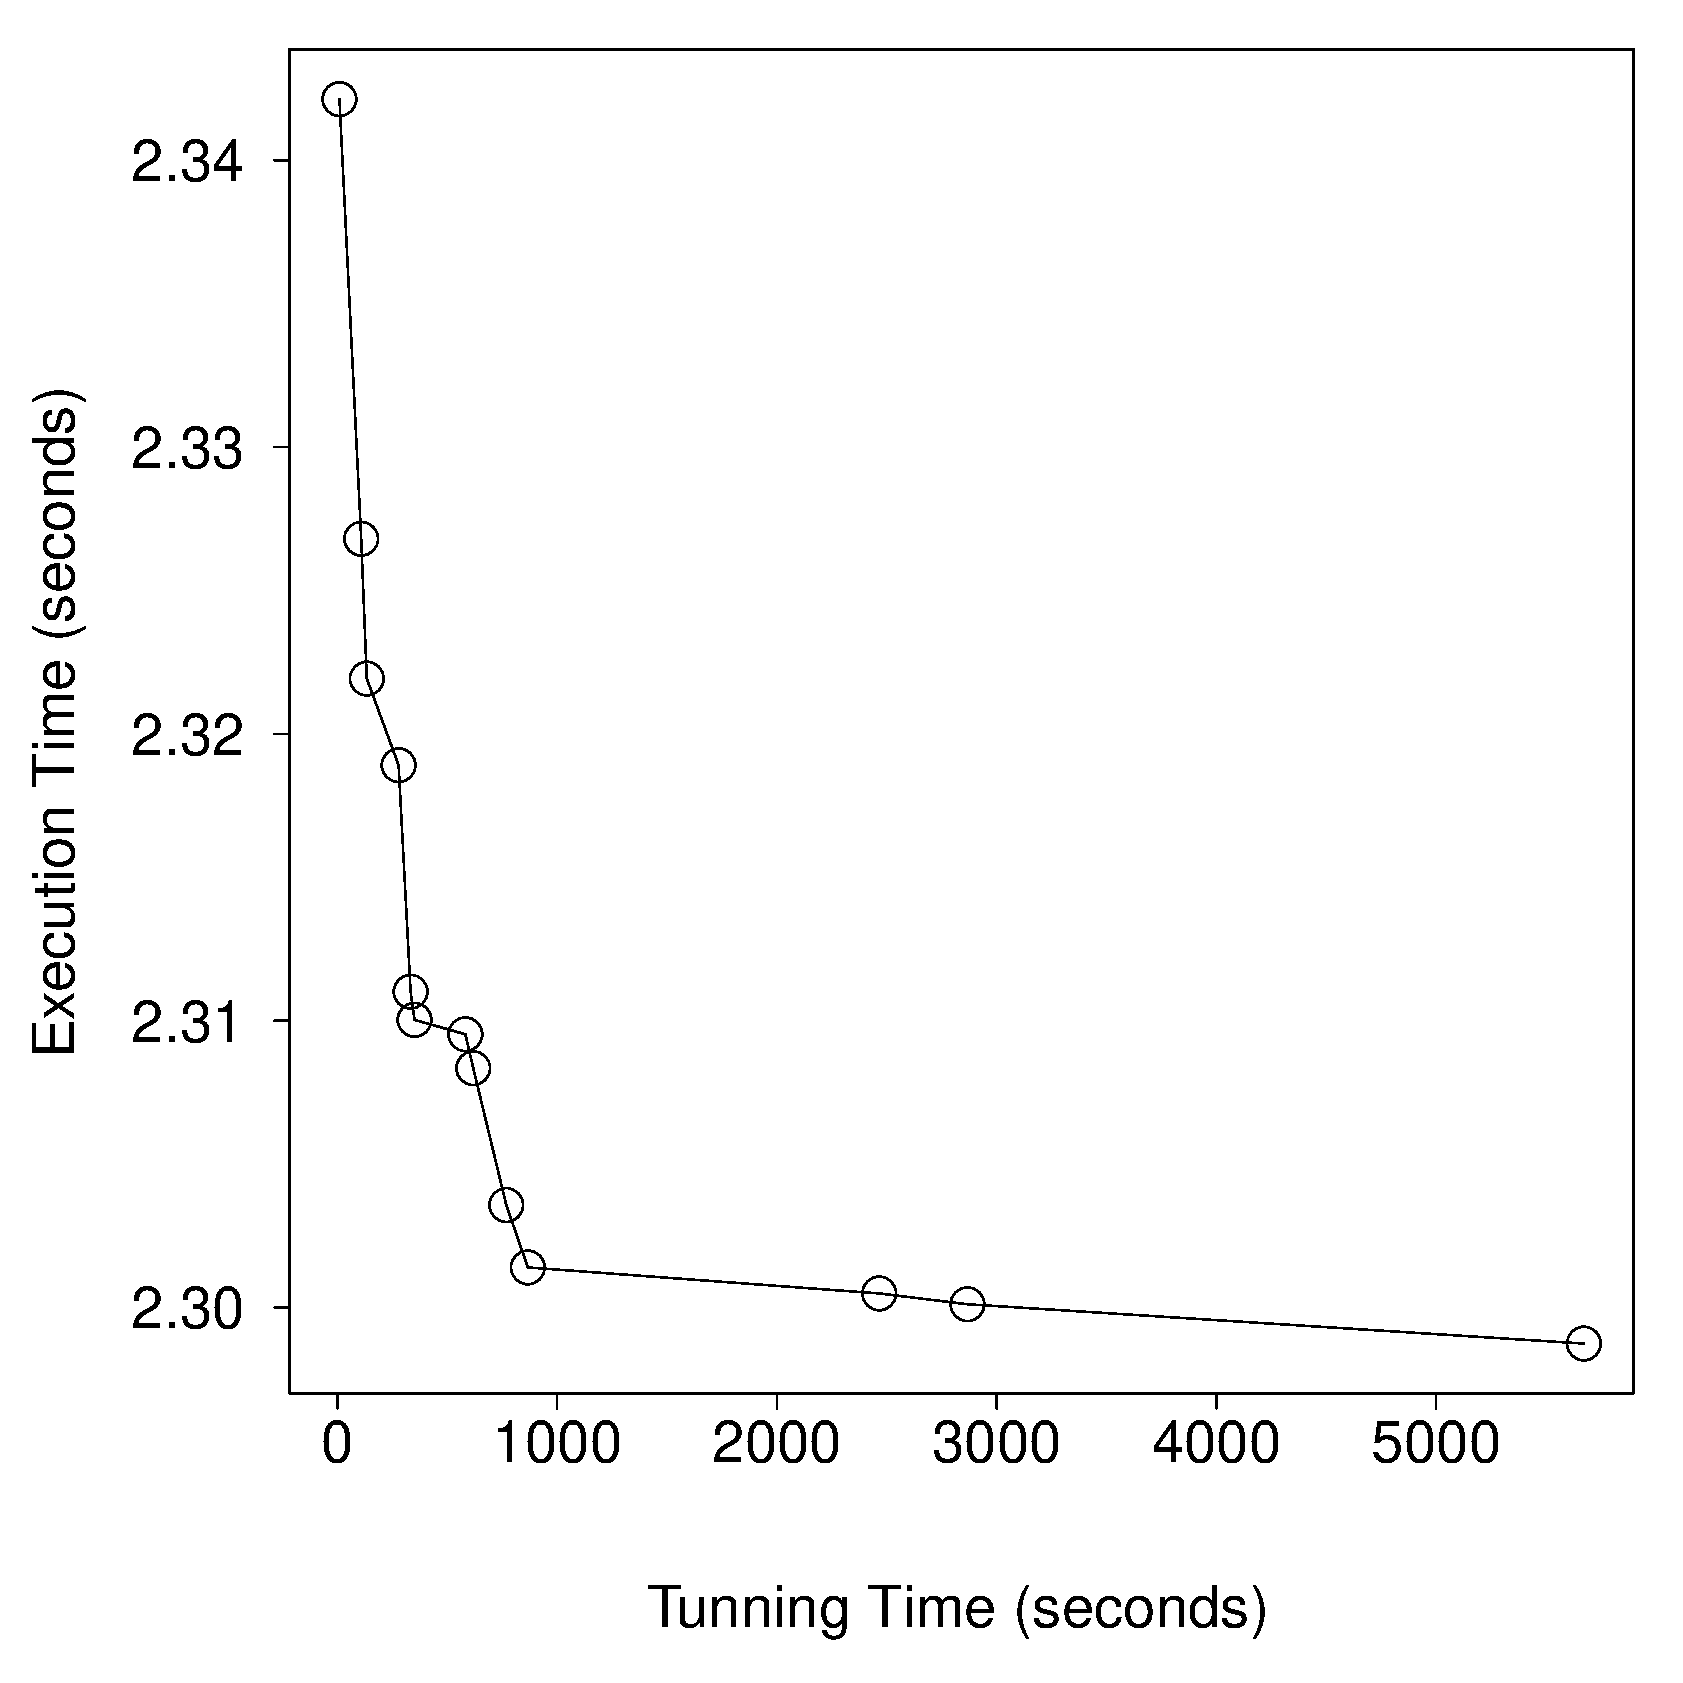
\includegraphics[scale=.22]{./images/heartwall-0-Tesla-K40-Best.eps}
        \caption{Best solutions found by the autotuner over time for the Heart Wall problem (HWL) in the Tesla K40}
        \label{fig:K40hwBest}
    \end{minipage}%
    \hfill
    \begin{minipage}{.48\textwidth}
        \centering
        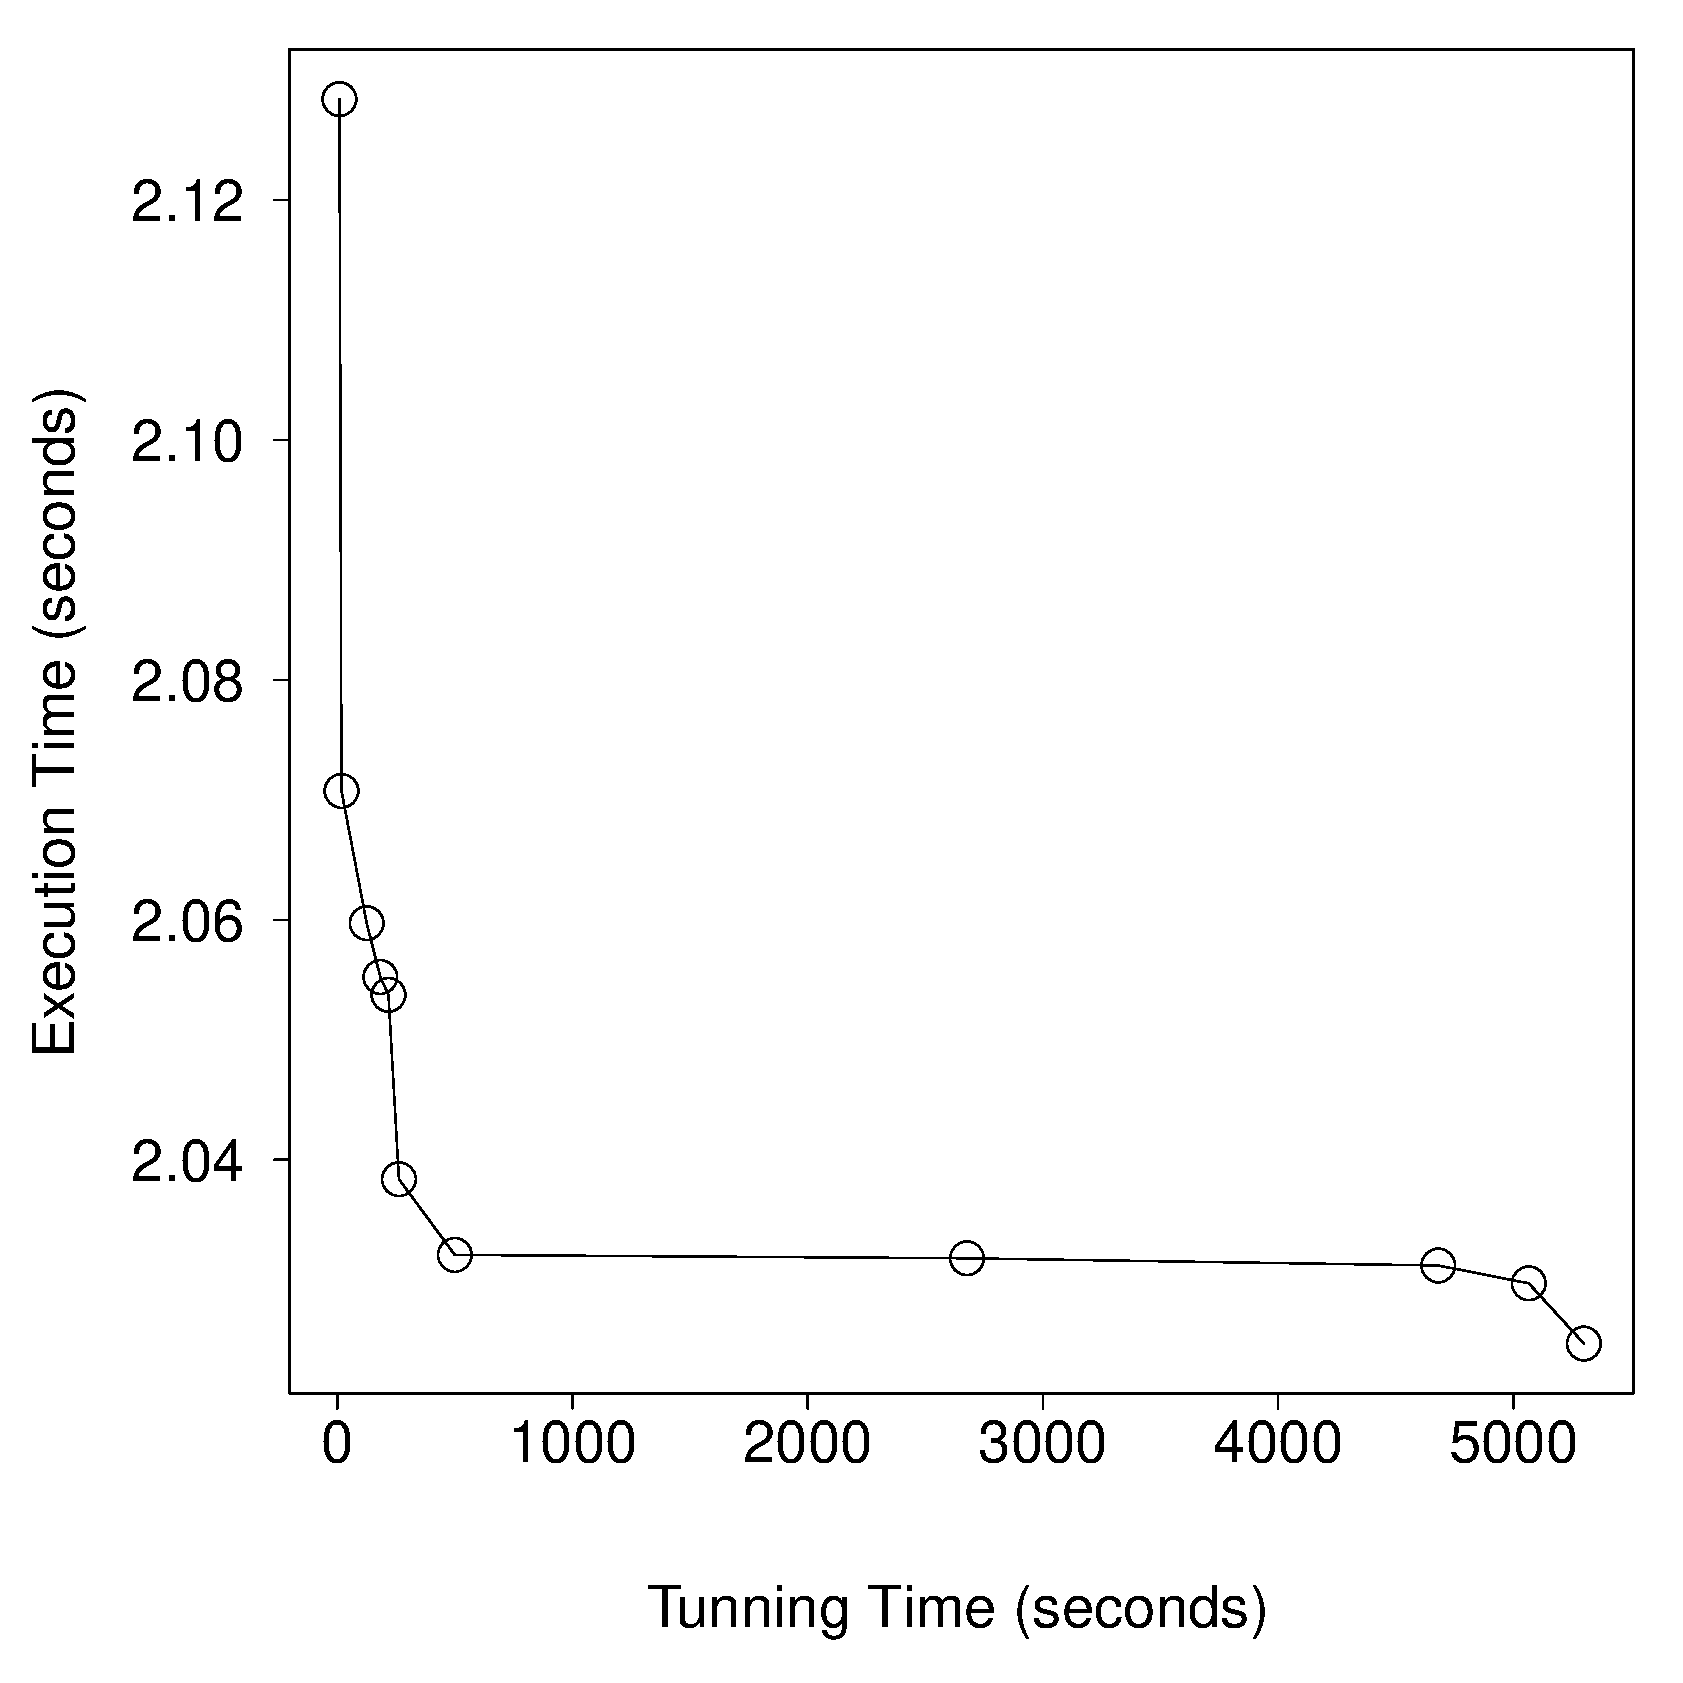
\includegraphics[scale=.22]{./images/gaussian-0-GTX-980-Best.eps}
        \caption{Best solutions found by the autotuner over time for the Gaussian Elimination problem (GAU) in the GTX 980}
        \label{fig:980gauBest}
    \end{minipage}%

    \begin{minipage}{.48\textwidth}
        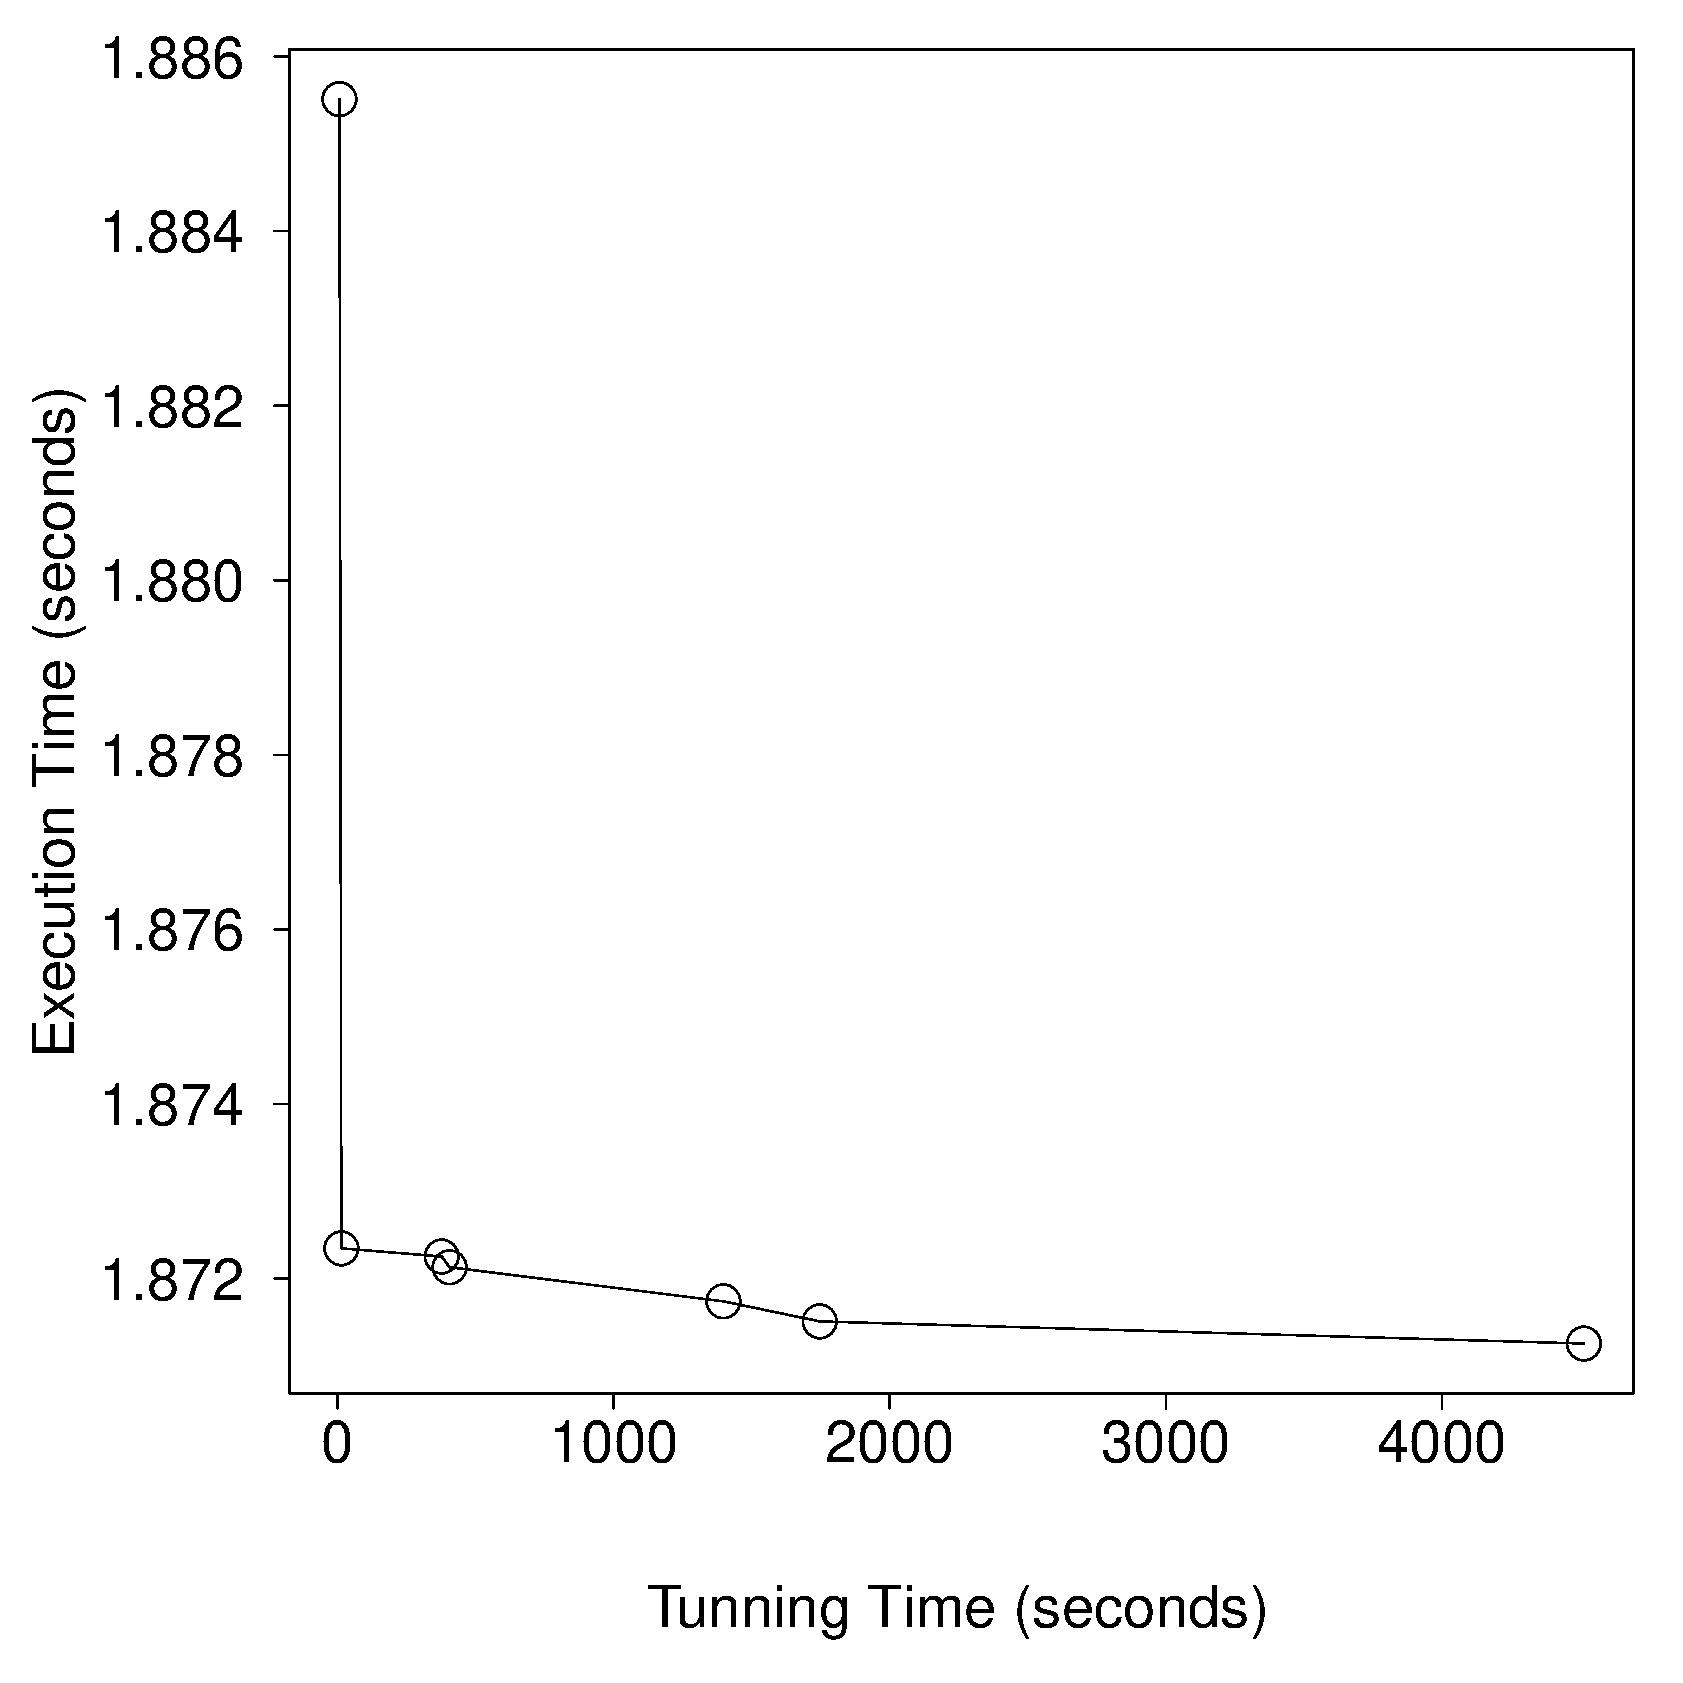
\includegraphics[scale=.22]{./images/Pathfinder-0-Tesla-K40-Best.eps}
        \caption{Best solutions found by the autotuner over time for the Path Finder problem (PTF) in the Tesla K40}
        \label{fig:K40ptfBest}
    \end{minipage}%
    \hfill
    \begin{minipage}{.48\textwidth}
        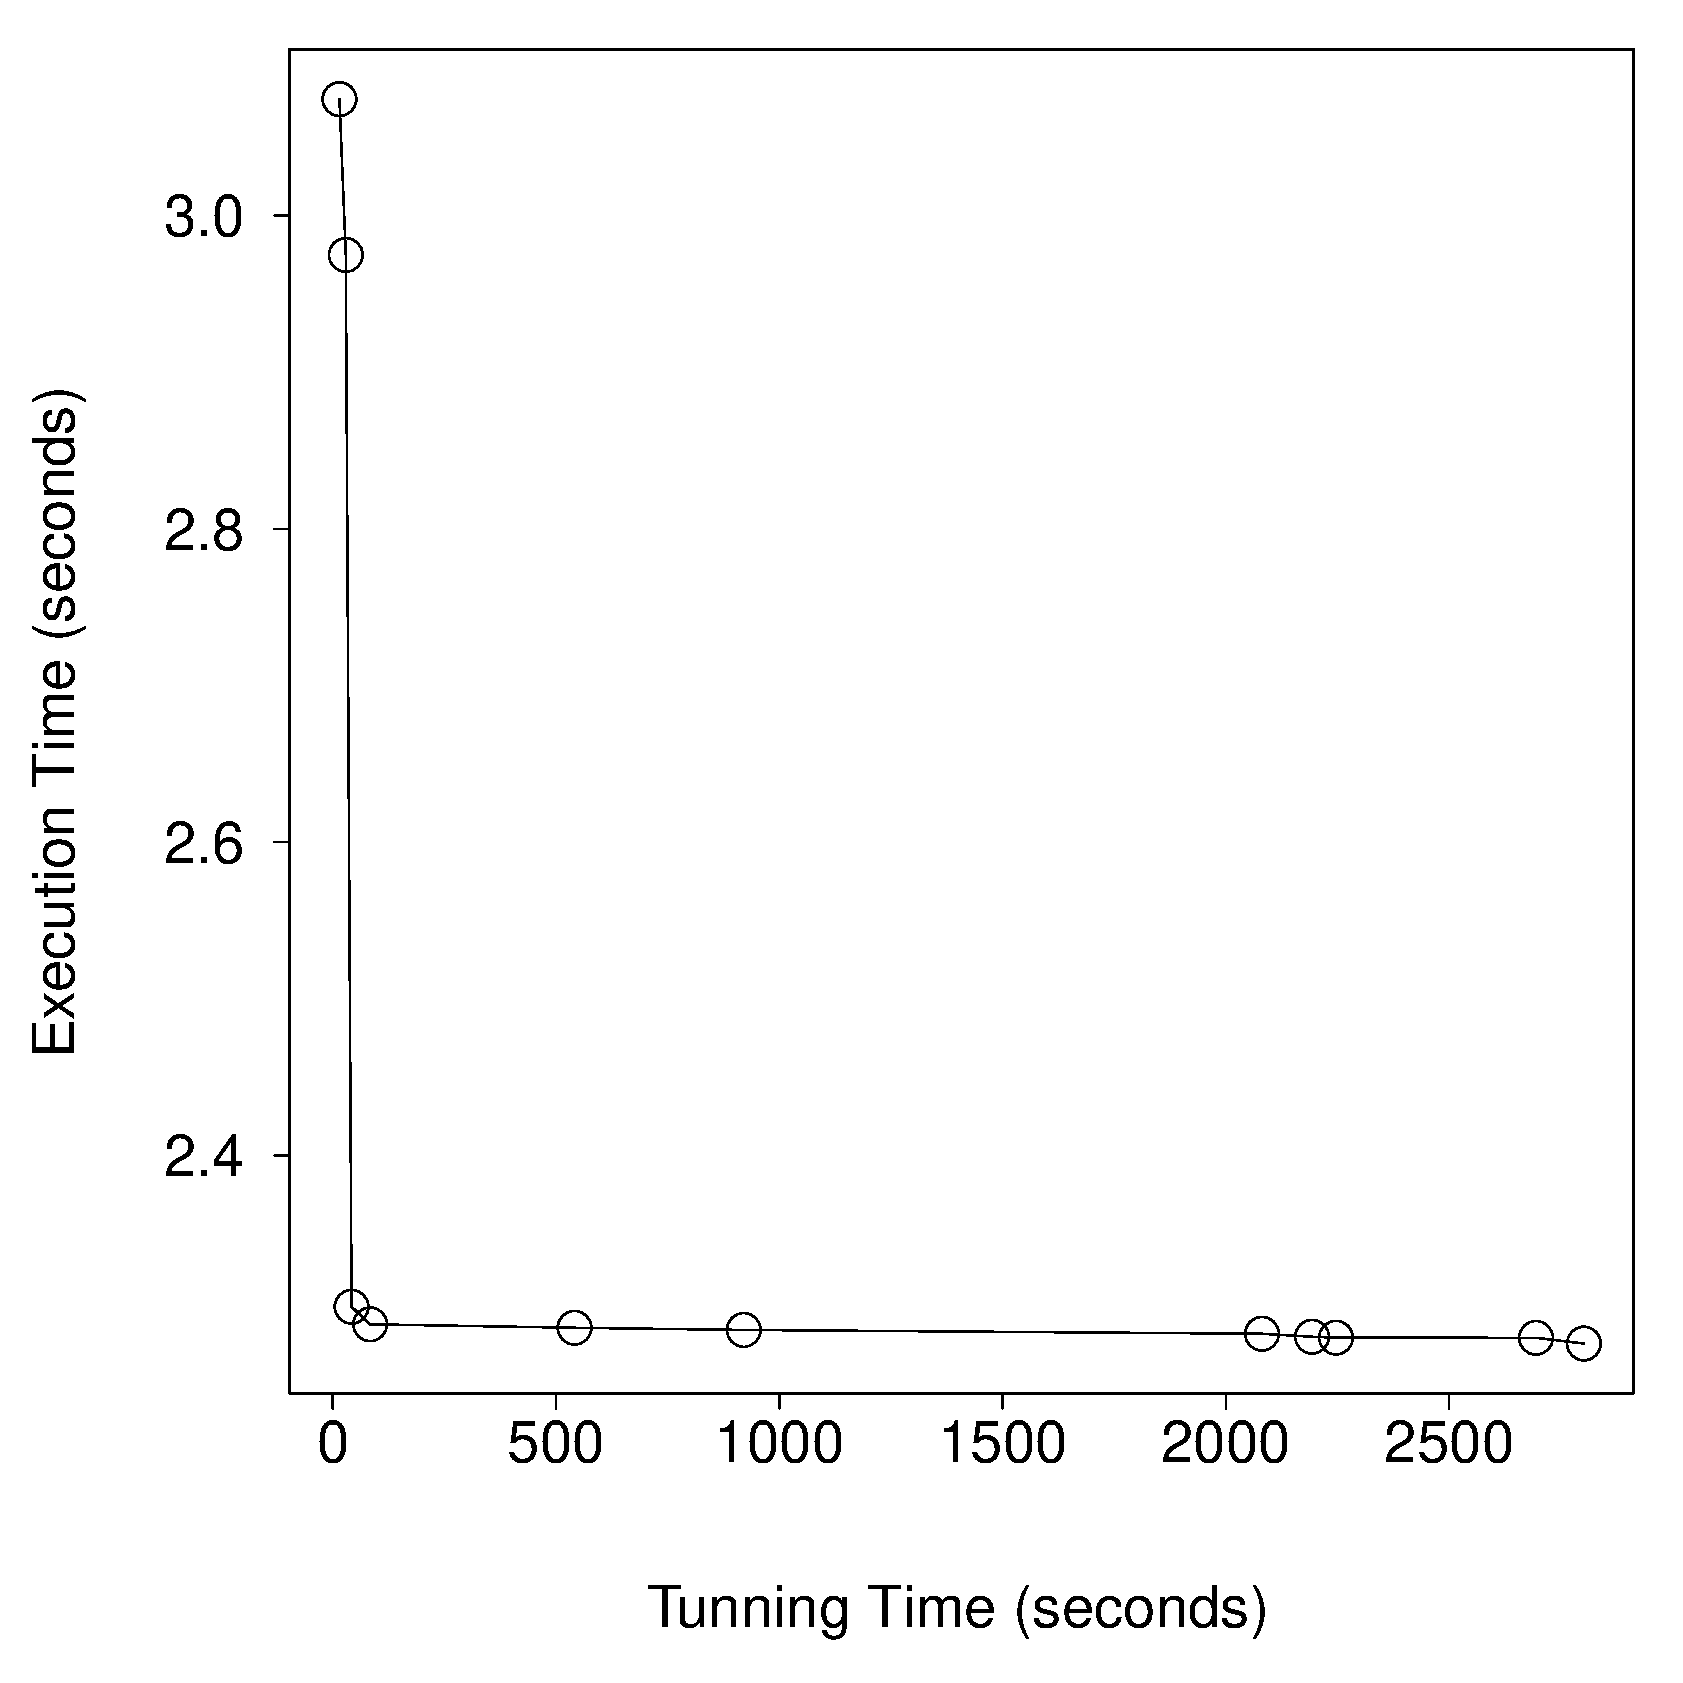
\includegraphics[scale=.22]{./images/myocyte-0-Tesla-K40-Best.eps}
        \caption{Best solutions found by the autotuner over time for the Myocyte problem (MYO) in the Tesla K40}
        \label{fig:K40myoBest}
    \end{minipage}
\end{figure}

Note that the autotuner is able to quickly improve upon the initial random
configuration, but the rate of improvement decays over tuning time. The
duration of all tuning runs was two hours, or 7200 seconds.  The rightmost
point in each graph represents the performance of the last improving
configuration found by the autotuner. After the tuning time of this
configuration, the autotuner did not find any improving configuration until the
end of its tuning run.

The autotuner used the mean of 10 performance measurements of a given
configuration as the fitness value, reducing fluctuations and improving the
measurement's accuracy. This is reflected in the proximity of the measurements
reported by the autotuner during tuning, shown in figures~\ref{fig:K40hwBest},
\ref{fig:980gauBest}, \ref{fig:K40ptfBest} and \ref{fig:K40myoBest} and the
mean values of 10 measurements of the final solution, shown in the
corresponding figures~\ref{fig:K40hwl}, \ref{fig:980gau}, \ref{fig:K40ptf} and
\ref{fig:K40myo}.

\subsubsection{Parameter Selection}

\begin{table}[htpb]
    \centering
    \footnotesize
    \begin{tabular}{ccc}
        \toprule
        \textbf{Flag} & \textbf{Cluster 0 (17\%)} & \textbf{Cluster 1 (83\%)} \\\midrule
        no-align-double               & on     & on     \\\midrule
        use\_fast\_math               & on     & on     \\\midrule
        preserve-relocs               & off    & off    \\\midrule
        relocatable-device-code       & true   & false  \\\midrule
        ftz                           & true   & true   \\\midrule
        prec-div                      & true   & false  \\\midrule
        prec-sqrt                     & true   & true   \\\midrule
        fmad                          & false  & false  \\\midrule
        allow-expensive-optimizations & false  & true   \\\midrule
        gpu-architecture              & sm\_20 & sm\_50 \\\midrule
        def-load-cache                & cv     & ca     \\\midrule
        opt-level                     & 1      & 3      \\\midrule
        maxrregcount                  & 42     & 44.6   \\\bottomrule
        \end{tabular}
    \caption{Parameter clusters for all Rodinia problems in the GTX 750}
    \label{tab:750RodiniaClusters}
\end{table}

We attempted to associate compilation parameters to applications and GPUs using
WEKA's~\cite{holmes1994weka} clustering algorithms. Although we could not find
significant relations for most applications we detected that the
\texttt{ftz=true} in MMS and the Compute Capabilities 3.0, 5.0 and 5.2 in GAU
caused the speedups observed in the GTX 980 for these applications.
Table~\ref{tab:750RodiniaClusters} shows clusters obtained with the K-means
WEKA algorithm for autotuned parameter sets for the Rodinia Benchmark in the
GTX 750. Unlike most clusters found for all GPUs and problems, these clusters
did not contain an equal number of instances. The difficulty of finding
associations between compiler optimizations, applications and GPUs justifies
the autotuning of compiler parameters in the general case.


\subsection{Small Measurement Time}
\label{subsec:smalltime}

\subsection{Summary and Future Work}
\label{subsec:GPUconcl}

We used the OpenTuner framework to implement an autotuner for the search space
defined by the parameters of the CUDA compiler. We composed a benchmark of 17
heterogeneous applications and compared their performance in one Kepler and two
Maxwell microarchitecture GPUs.  Although the autotuner often beat the
compiler’s high-level optimizations it still underperformed for some problems.
We achieved over 2x speedup for Gaussian Elimination (GAU) and almost 2x
speedup for Heart Wall (HWL),  and over 4x speedup for a matrix multiplication
algorithm (MMS).

This paper showed that it is possible to improve the performance of GPU
applications applying empirical and automatic tuning techniques. Our results
and clustering attempts emphasize the importance of automatic optimization
techniques by showing that different compilation options have to be selected in
order to achieve performance improvements in different GPUs and that it is
difficult to associate compiler optimization parameters, applications and GPUs.

Future work will include application parameters and options for the GCC
compiler, which also composes the CUDA compilation chain.  We would also like
to apply the Programming by Optimization~\cite{hoos2012programming} design
paradigm for GPU and parallel programming. We will continue to apply clustering
algorithms to future experiments and we will perform more comprehensive
experiments to explore the search space of CUDA compiler parameters. We hope
these approaches will enable us to provide valuable guidelines for CUDA
parameter selection in the future.

To the best of our knowledge, this is the first work that applied autotuning
techniques to CUDA compiler parameters for GPU applications using the OpenTuner
framework, comparing the speedup achieved in different GPU architectures for
heterogeneous applications.



\section{Autotuning and Distributed Computing}
\label{sec:autotuningCloud}

\subsection{Introduction}
\label{subsec:CLintro}

\subsection{Results}
\label{subsec:CLres}

\subsection{Parallel and Distributed Programming in OpenTuner}
\label{subsec:parallel}

\subsection{Summary and Future Work}
\label{subsec:CLconcl}

\section{Selecting Parameters for High-Level Synthesis for FPGAs}
\label{sec:paramSelFPGA}

\subsection{Introduction}
\label{subsec:FPGAintro}

\subsection{Results}
\label{subsec:FPGAres}

\subsection{Large Measurement Time}
\label{subsec:bigtime}

\subsection{Summary and Future Work}
\label{subsec:FPGAconcl}

\section{Configuring Hardware and Software for the Dot Product Engine}
\label{sec:configDPE}

\subsection{Introduction}
\label{subsec:DPEintro}

\subsection{Results}
\label{subsec:DPEres}

\subsection{Summary and Future Work}
\label{subsec:DPEconcl}
